%%%%%%%%%%%%%%%%%%%%%%%%%%%%%%%%%%%%%%%%%%%%%%%%%%%%%%%%%%%%%%%%%%%%%%%%%%%%%%%%
% PREAMBLE
%%%%%%%%%%%%%%%%%%%%%%%%%%%%%%%%%%%%%%%%%%%%%%%%%%%%%%%%%%%%%%%%%%%%%%%%%%%%%%%%
\documentclass[12pt, a4paper, ukenglish]{article}

% -------------------------- Font and Encoding ---------------------------------
\usepackage[T1]{fontenc}
\usepackage{times} % Use Times font
\usepackage[utf8]{inputenc}

% -------------------------- Page Layout ---------------------------------------
\usepackage[left=2.5cm, top=2cm, right=2.5cm, bottom=2cm]{geometry}
\setlength{\parskip}{\medskipamount}

% -------------------------- Required Packages ---------------------------------
\usepackage{amsmath,amssymb}  % Combined for faster loading
\usepackage{graphicx}
\usepackage{mathtools}        % Loads amsmath automatically, provides advanced features
\usepackage{longtable,booktabs}  % Combined table packages
\usepackage{pdfpages}
% Specialized math packages (load only if needed)
\usepackage{cancel,esint,mathdots,stmaryrd}
\usepackage[version=4]{mhchem}
\usepackage{stackrel}
% \usepackage[ukenglish]{babel}

% -------------------------- Bibliography Settings -----------------------------
% NOTE: The 'cite' package conflicts with biblatex. It has been removed.
\usepackage[style=ieee, backend=biber]{biblatex}
\addbibresource{final_report.bib} % Make sure this filename matches your .bib file

% -------------------------- Colors -------------------------------
\usepackage{xcolor} % Colours for hyperref package
% Define links colour
\newcommand{\linksColour}{black}

% -------------------- Header and Footer Settings ------------------------------
\usepackage{fancyhdr}
\pagestyle{fancy}
\fancyhead{}                   % clear the default header
\fancyfoot{}                   % clear the default footer
% \fancyfoot[CO,CE]{\footnotesize\thepage}   % page number in the middle
\renewcommand{\headrulewidth}{0.0pt}       % remove the default header line
% Header and footer of automatically generated pages (e.g. TOC)
\fancypagestyle{plain}{
    \fancyhead{}
    \fancyfoot{}
    % \fancyfoot[CO,CE]{\footnotesize\thepage}
    \renewcommand{\headrulewidth}{0pt}
}

% ------------------------ Title Page Box Settings -----------------------------
% settings for the text box on the front page
\newcommand\HRule{\noindent\rule{\linewidth}{2pt}}

% -------------------------- Figures Settings ----------------------------------
% Redefine how latex deals with figure placement
\renewcommand{\topfraction}{.85}
\renewcommand{\bottomfraction}{.7}
\renewcommand{\textfraction}{.15}
\renewcommand{\floatpagefraction}{.66}
\renewcommand{\dbltopfraction}{.66}
\renewcommand{\dblfloatpagefraction}{.66}
\usepackage[labelfont={bf,footnotesize},textfont={footnotesize}, labelsep=quad]{caption}

% ------------------------------ TOC Settings ----------------------------------
% Adding dots to sections in table of contents
\usepackage{tocloft}
\renewcommand{\cftloftitlefont}{\large\bfseries}
\renewcommand{\cftlottitlefont}{\large\bfseries}
\renewcommand{\cftsecleader}{\cftdotfill{\cftdotsep}}
% Adding the word Figure in list of figures
\renewcommand*\cftfigpresnum{Figure~}
\settowidth{\cftfignumwidth}{\cftfigpresnum}
\renewcommand{\cftfigaftersnumb}{\qquad}
% Adding the word Table in list of figures
\renewcommand*\cfttabpresnum{Table~}
\settowidth{\cfttabnumwidth}{\cfttabpresnum}
\renewcommand{\cfttabaftersnumb}{\qquad}
\setcounter{secnumdepth}{3}
\setcounter{tocdepth}{3}

% -------------------- Formatting Section Titles -------------------------------
% Shrinking the space after headers
\usepackage[clearempty]{titlesec} % loaded with a setting for automatically generated empty pages to be completely blank
\beforetitleunit = 1pt
\aftertitleunit = 1pt
% specifying the spacing before and after the titles (note \parskip = 9pts)
\titlespacing{\section}{0pt}{*9}{*9}    % for 18 pt space
\titlespacing{\subsection}{0pt}{*3}{*3}  % for 12 pt space
\titlespacing{\subsubsection}{0pt}{*3}{*3} % for 12 pt space
% specifying the title formatting
\titleformat{\section} {\normalfont\fontsize{14}{14}\bfseries}{\thesection.}{1em}{}
\titleformat{\subsection} {\normalfont\fontsize{12}{12}\bfseries}{\thesubsection}{1em}{}
\titleformat{\subsubsection} {\normalfont\fontsize{12}{12}\it}{\thesubsubsection}{1em}{}

% Modifying how appendices look (title and toc)
\usepackage[titletoc,title]{appendix}

% ------------------------- Nomenclature Settings ------------------------------
\usepackage{nomencl}
\makenomenclature
\def\nompreamble{\addcontentsline{toc}{section}{\nomname}\markboth{\nomname}{\nomname}}
% customising nomenclature groups
\usepackage{ifthen}
\renewcommand{\nomgroup}[1]{
    \ifthenelse{\equal{#1}{A}}{\item[\textbf{Symbols}]}{%
    \ifthenelse{\equal{#1}{G}}{\item[\textbf{Greek Symbols}]}{}
    }% matches Greek Symbols
}% matches Roman Symbols
% unit column in nomenclature
\newcommand{\nomunit}[1]{\renewcommand{\nomentryend}{\hspace*{\fill}#1}}

% -------------------------- Code Listings Settings ----------------------------
\usepackage{listings}
\lstset{
    basicstyle={\ttfamily\footnotesize},
    belowcaptionskip=3mm,
    breaklines=true,
    commentstyle={\color[rgb]{0,0.5,0}},
    frame=tb, % Top and bottom frame lines
    keywordstyle={\color{blue}},
    language=Matlab,
    numbers=left,
    numberstyle={\scriptsize},
    showstringspaces=false,
    stringstyle={\color{purple}}
}
% Change default name for code environments
\renewcommand{\lstlistingname}{Program}

% -------------------------- Miscellaneous Settings ----------------------------
\usepackage[british]{isodate}
\usepackage{menukeys}       % for menu instructions
\usepackage[bottom]{footmisc} % force footnotes to be always at the bottom of the page
\usepackage{multirow}
\usepackage{units}
\allowdisplaybreaks     % to allow page breaks within equations

% Disable automatic date printing
% \date{}

% -------------------------- Hyperlinks (LOAD LAST) -------------------------------
% hyperref package should be loaded near the end for optimal performance
\usepackage[colorlinks=true, linkcolor=\linksColour, citecolor=\linksColour, urlcolor=blue, bookmarksnumbered=true, bookmarksopen=true, bookmarksopenlevel=1]{hyperref}
\urlstyle{rm}               % Change url fonts to match report font

%%%%%%%%%%%%%%%%%%%%%
% REFERENCING OF IMAGES AND FIGURE
%%%%%%%%%%%%%%%%%%%%%%%%

%%%%%%%%%%%%%%%%%%%%%%%%
% IMAGES - Optimized for faster compilation
%%%%%%%%%%%%%%%%%%%%%%%%
\newcommand{\catImage}{
    \begin{figure}[ht]
        \centering
        
\includegraphics[width=0.3\linewidth]{figures/cat.jpg}
        \caption{Image of a cat used for testing the AlexNet model}
        \label{fig:cat}
    \end{figure}
}
%%%%%%%%%%%%%%%%%%%%%%%%
% FIGURES - Optimized placement
%%%%%%%%%%%%%%%%%%%%%%%%
\newcommand{\MACRegImage}{
    \begin{figure}[ht]
        \centering
        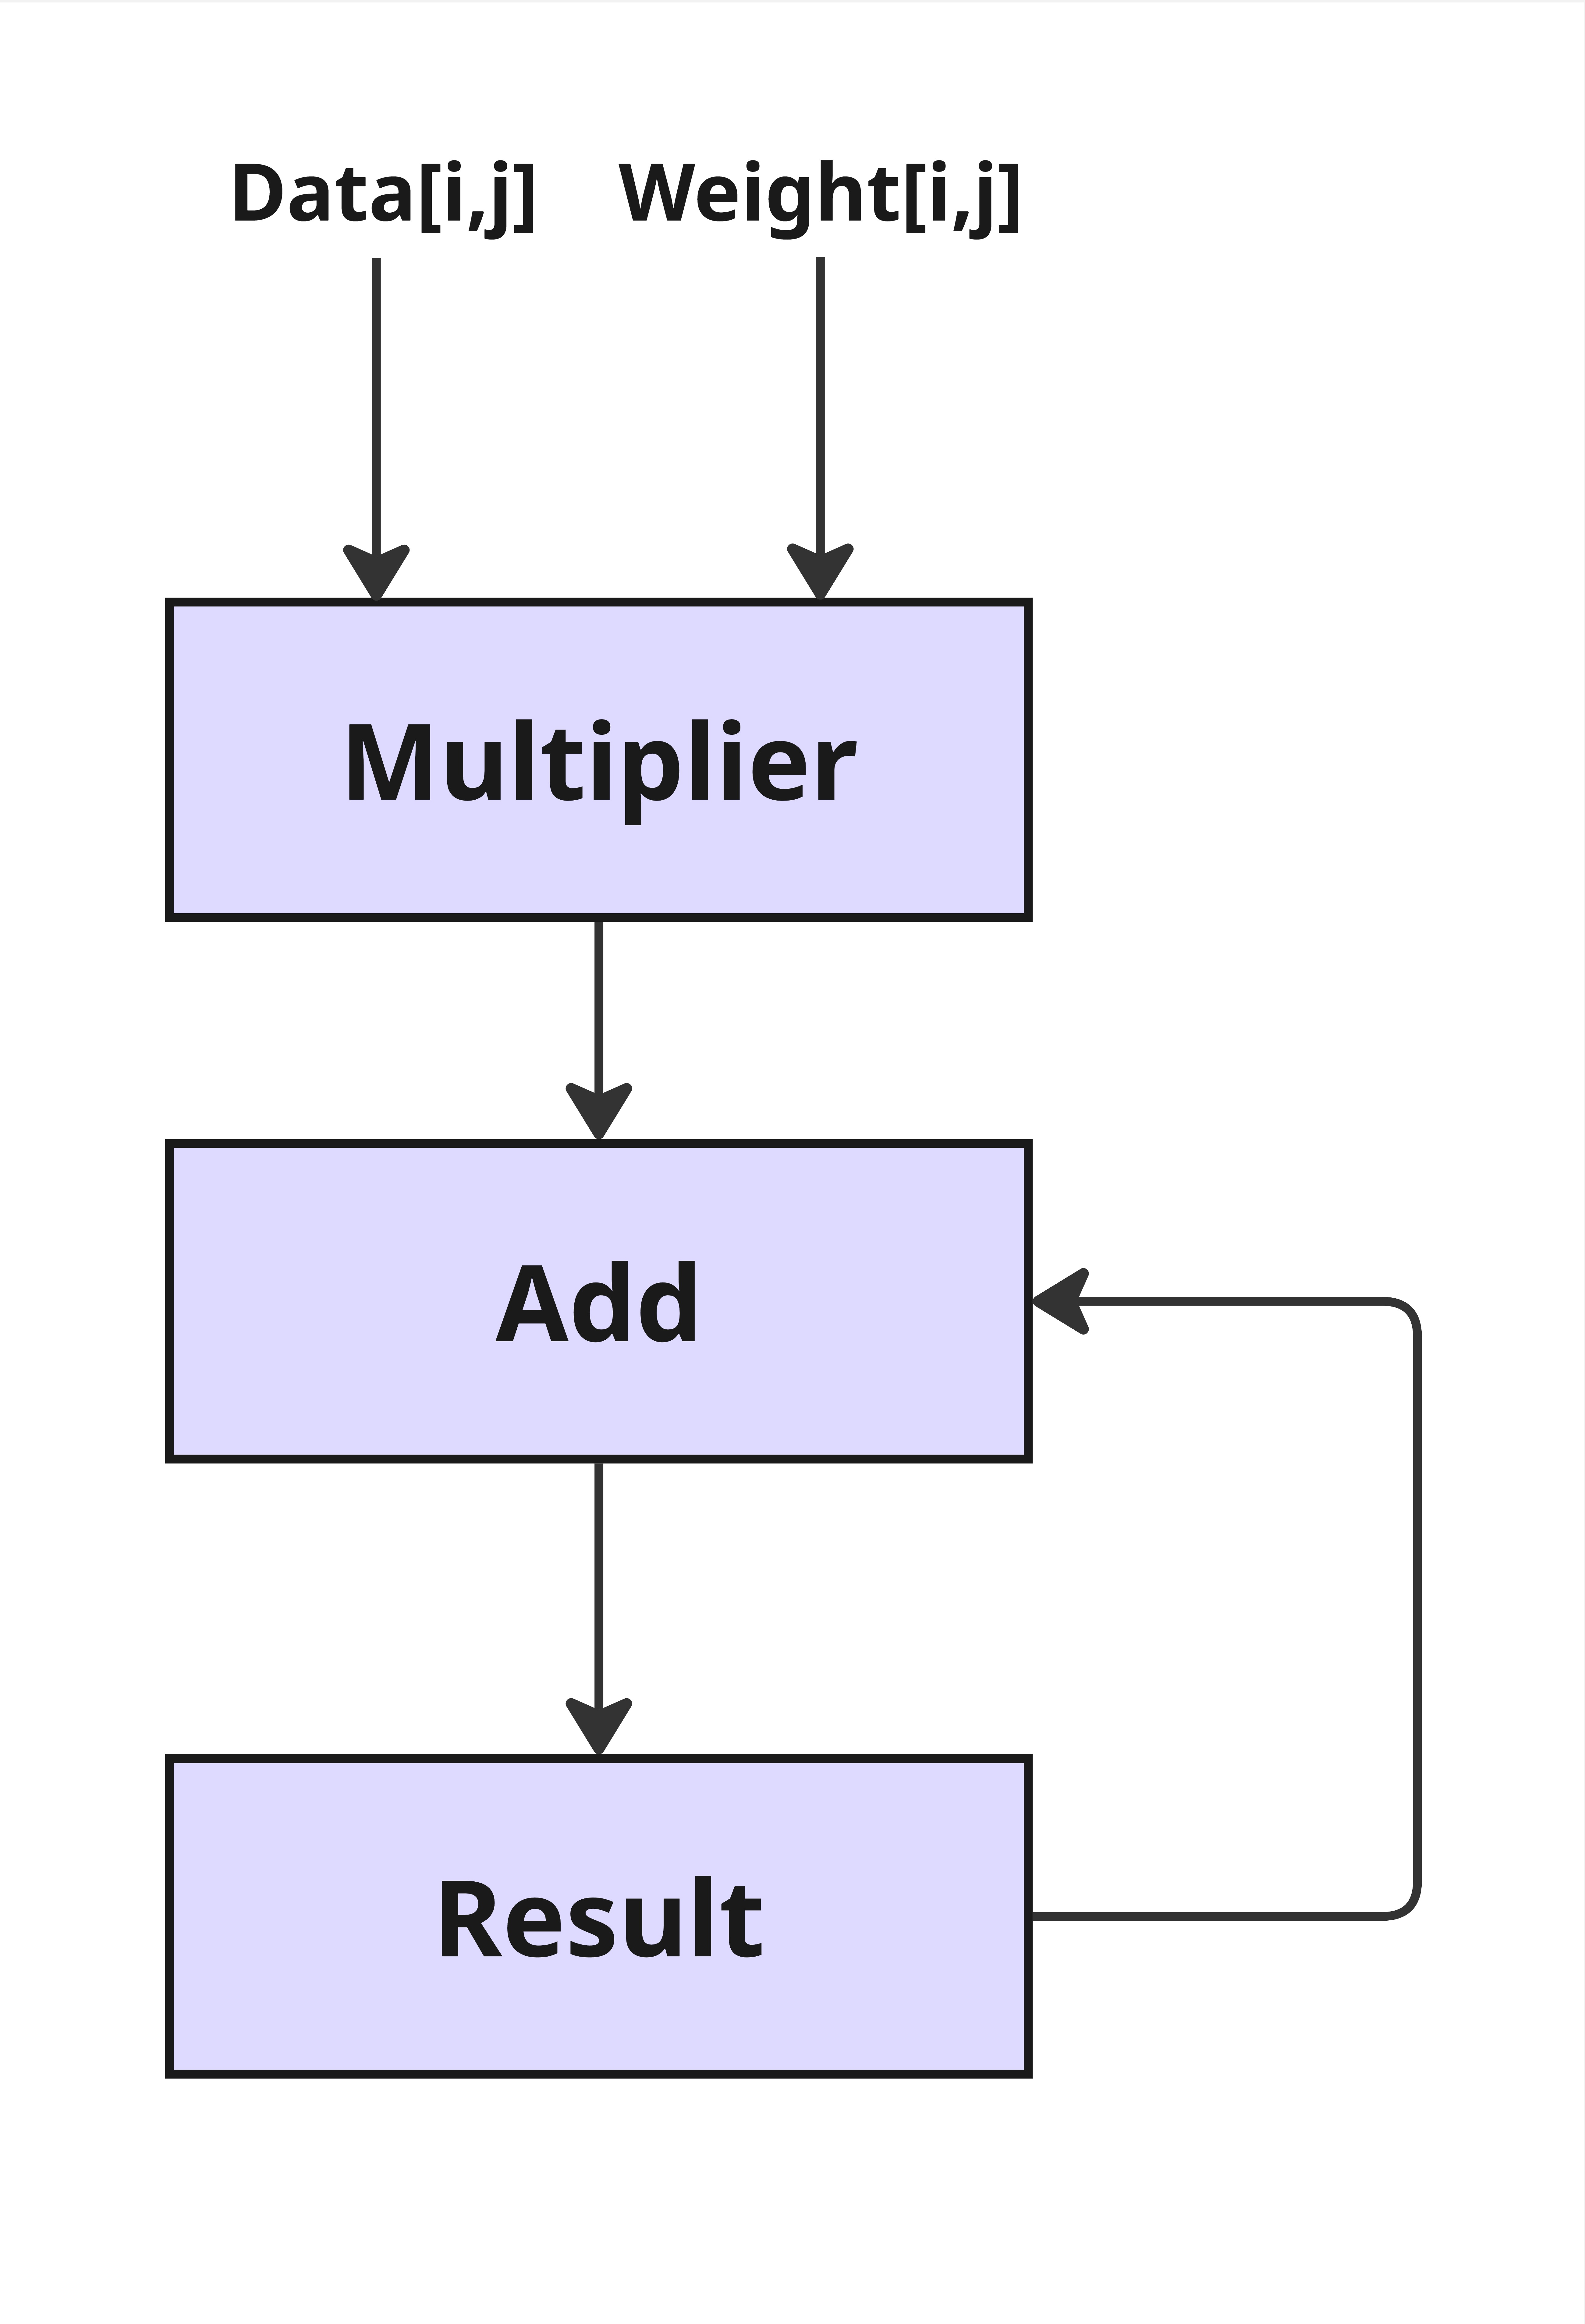
\includegraphics[width=0.2\linewidth]{figures/MAC.jpg}
        \caption{MAC unit in the Processing Element (PE)}
        \label{fig:MAC}
    \end{figure}
}
\newcommand{\baselineSystolicArrayImage}{
    \begin{figure}[ht]
        \centering
        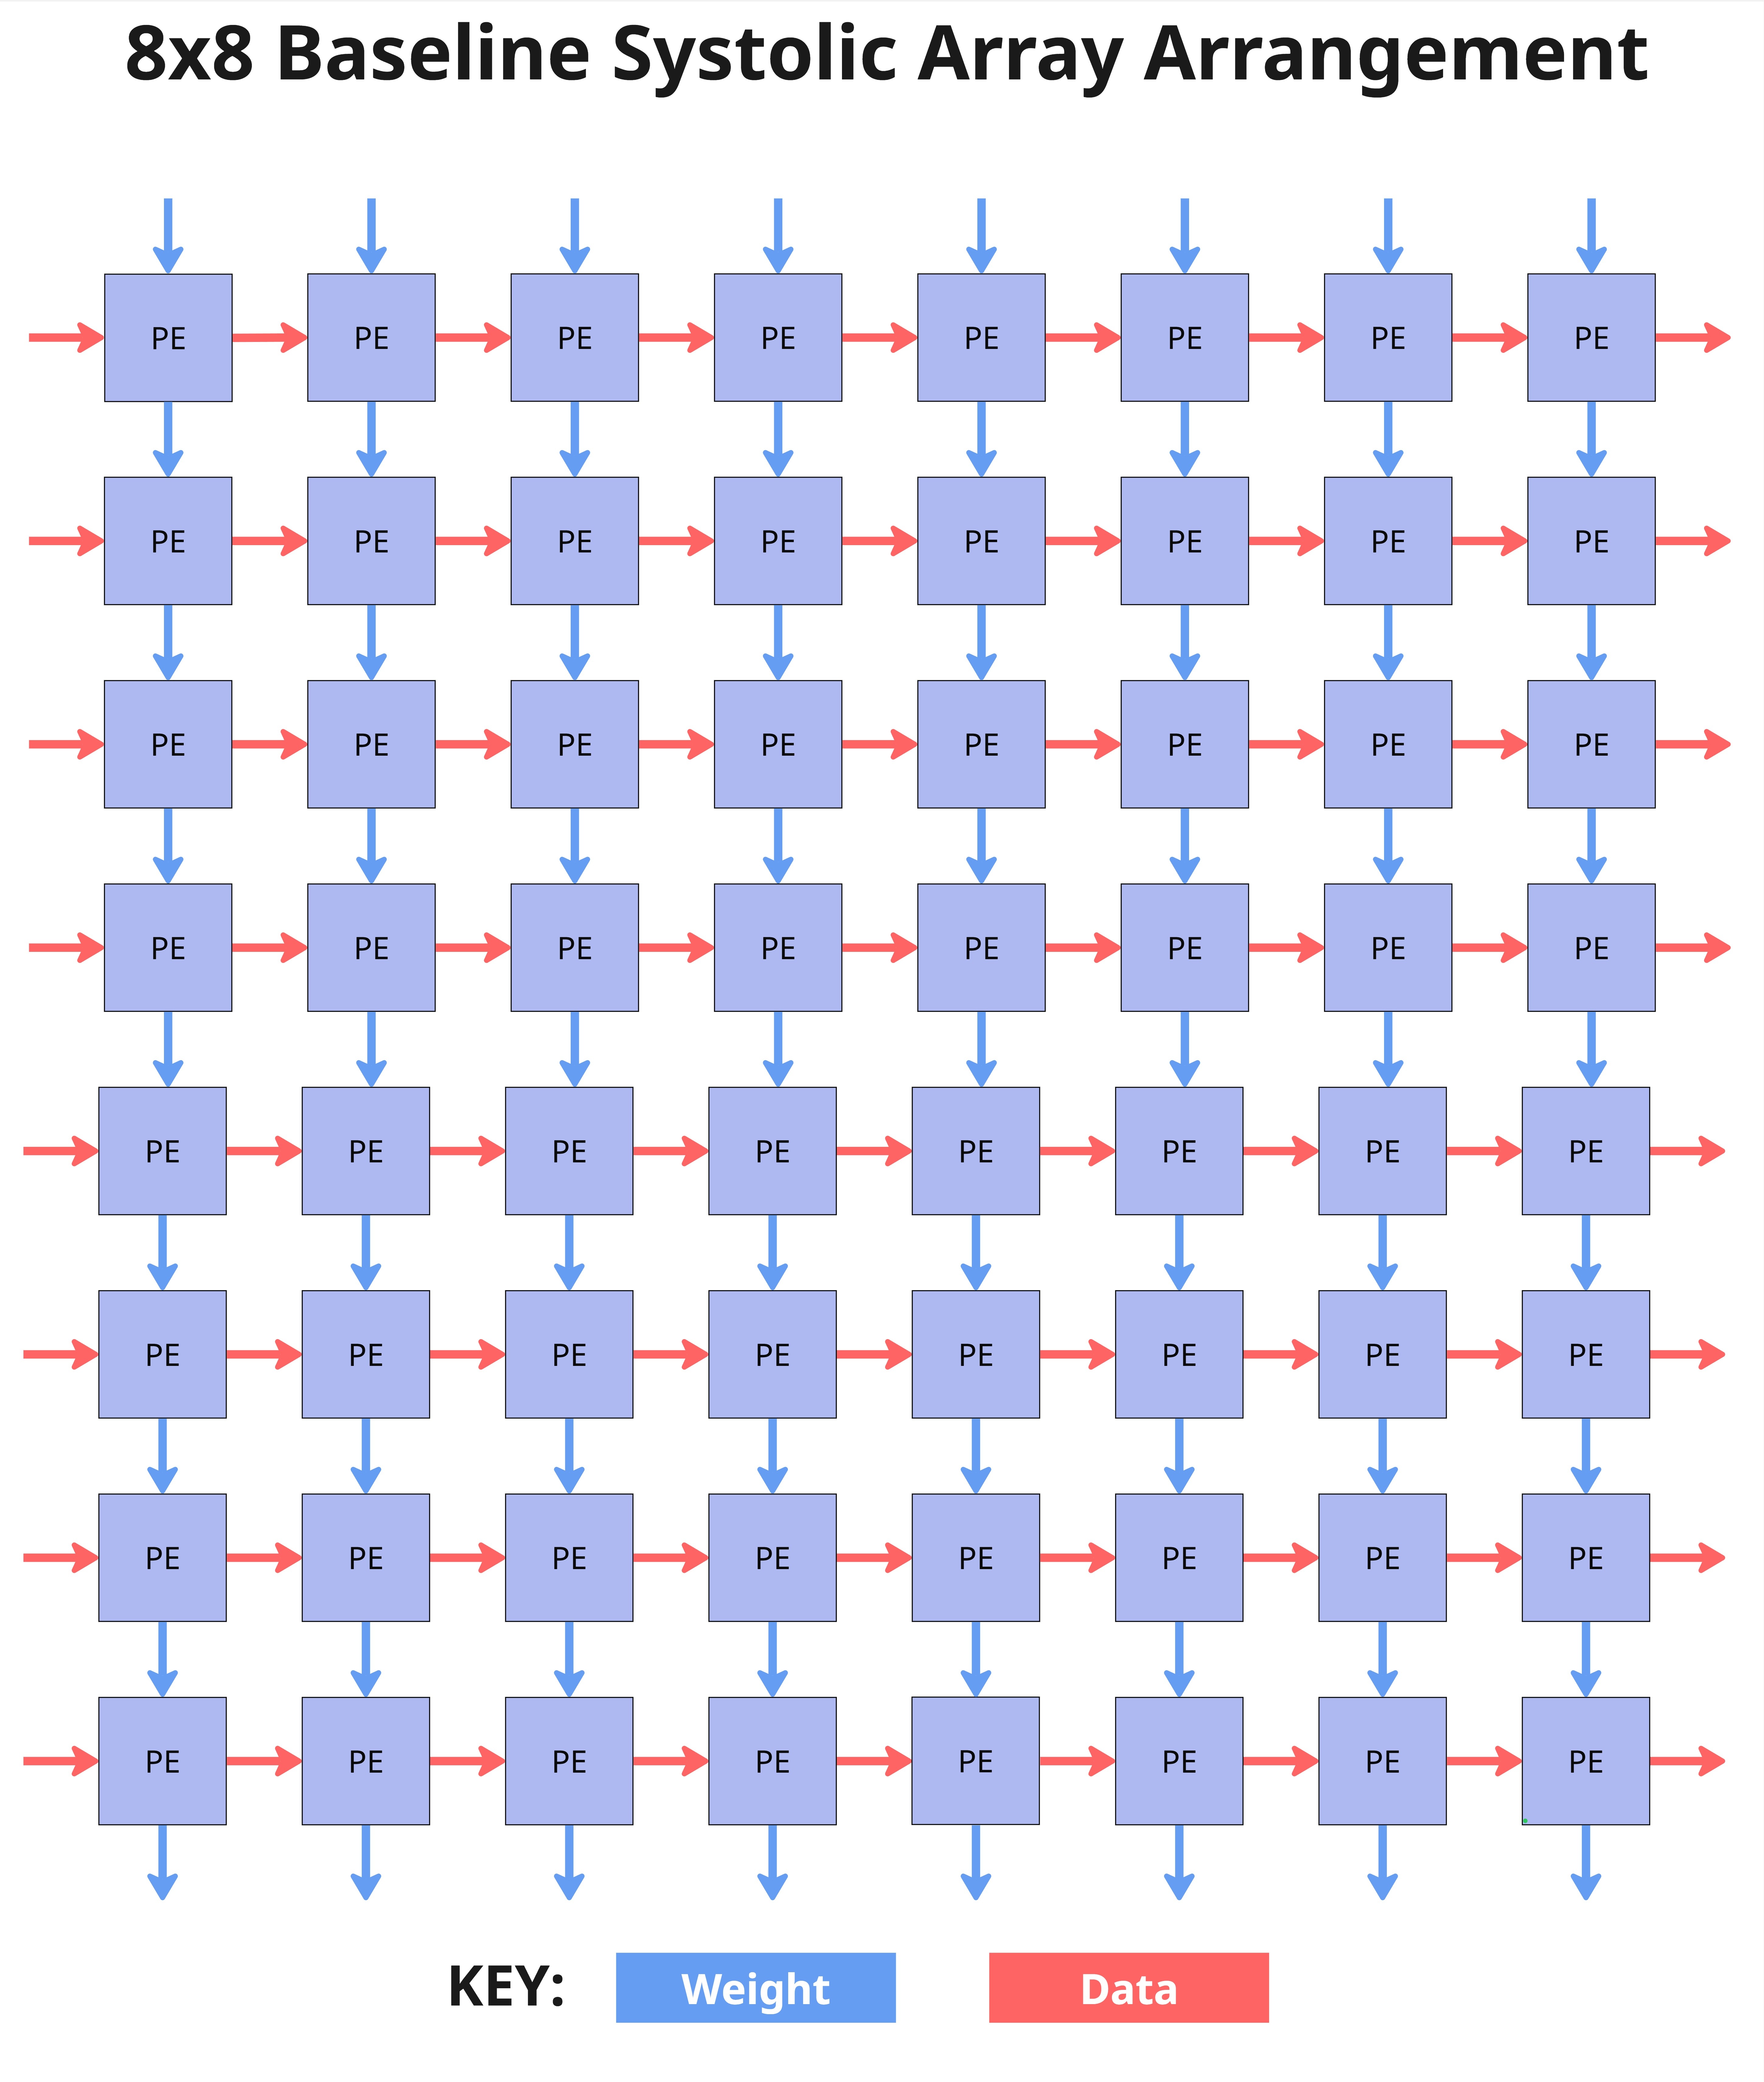
\includegraphics[width=0.4\linewidth]{figures/baseline_systolic_array.jpg}
        \caption{Baseline Systolic Array Arrangement}
        \label{fig:baseline_systolic_array}
    \end{figure}
}

\newcommand{\baselineDataflowImage}{
    \begin{figure}[ht]
        \centering
        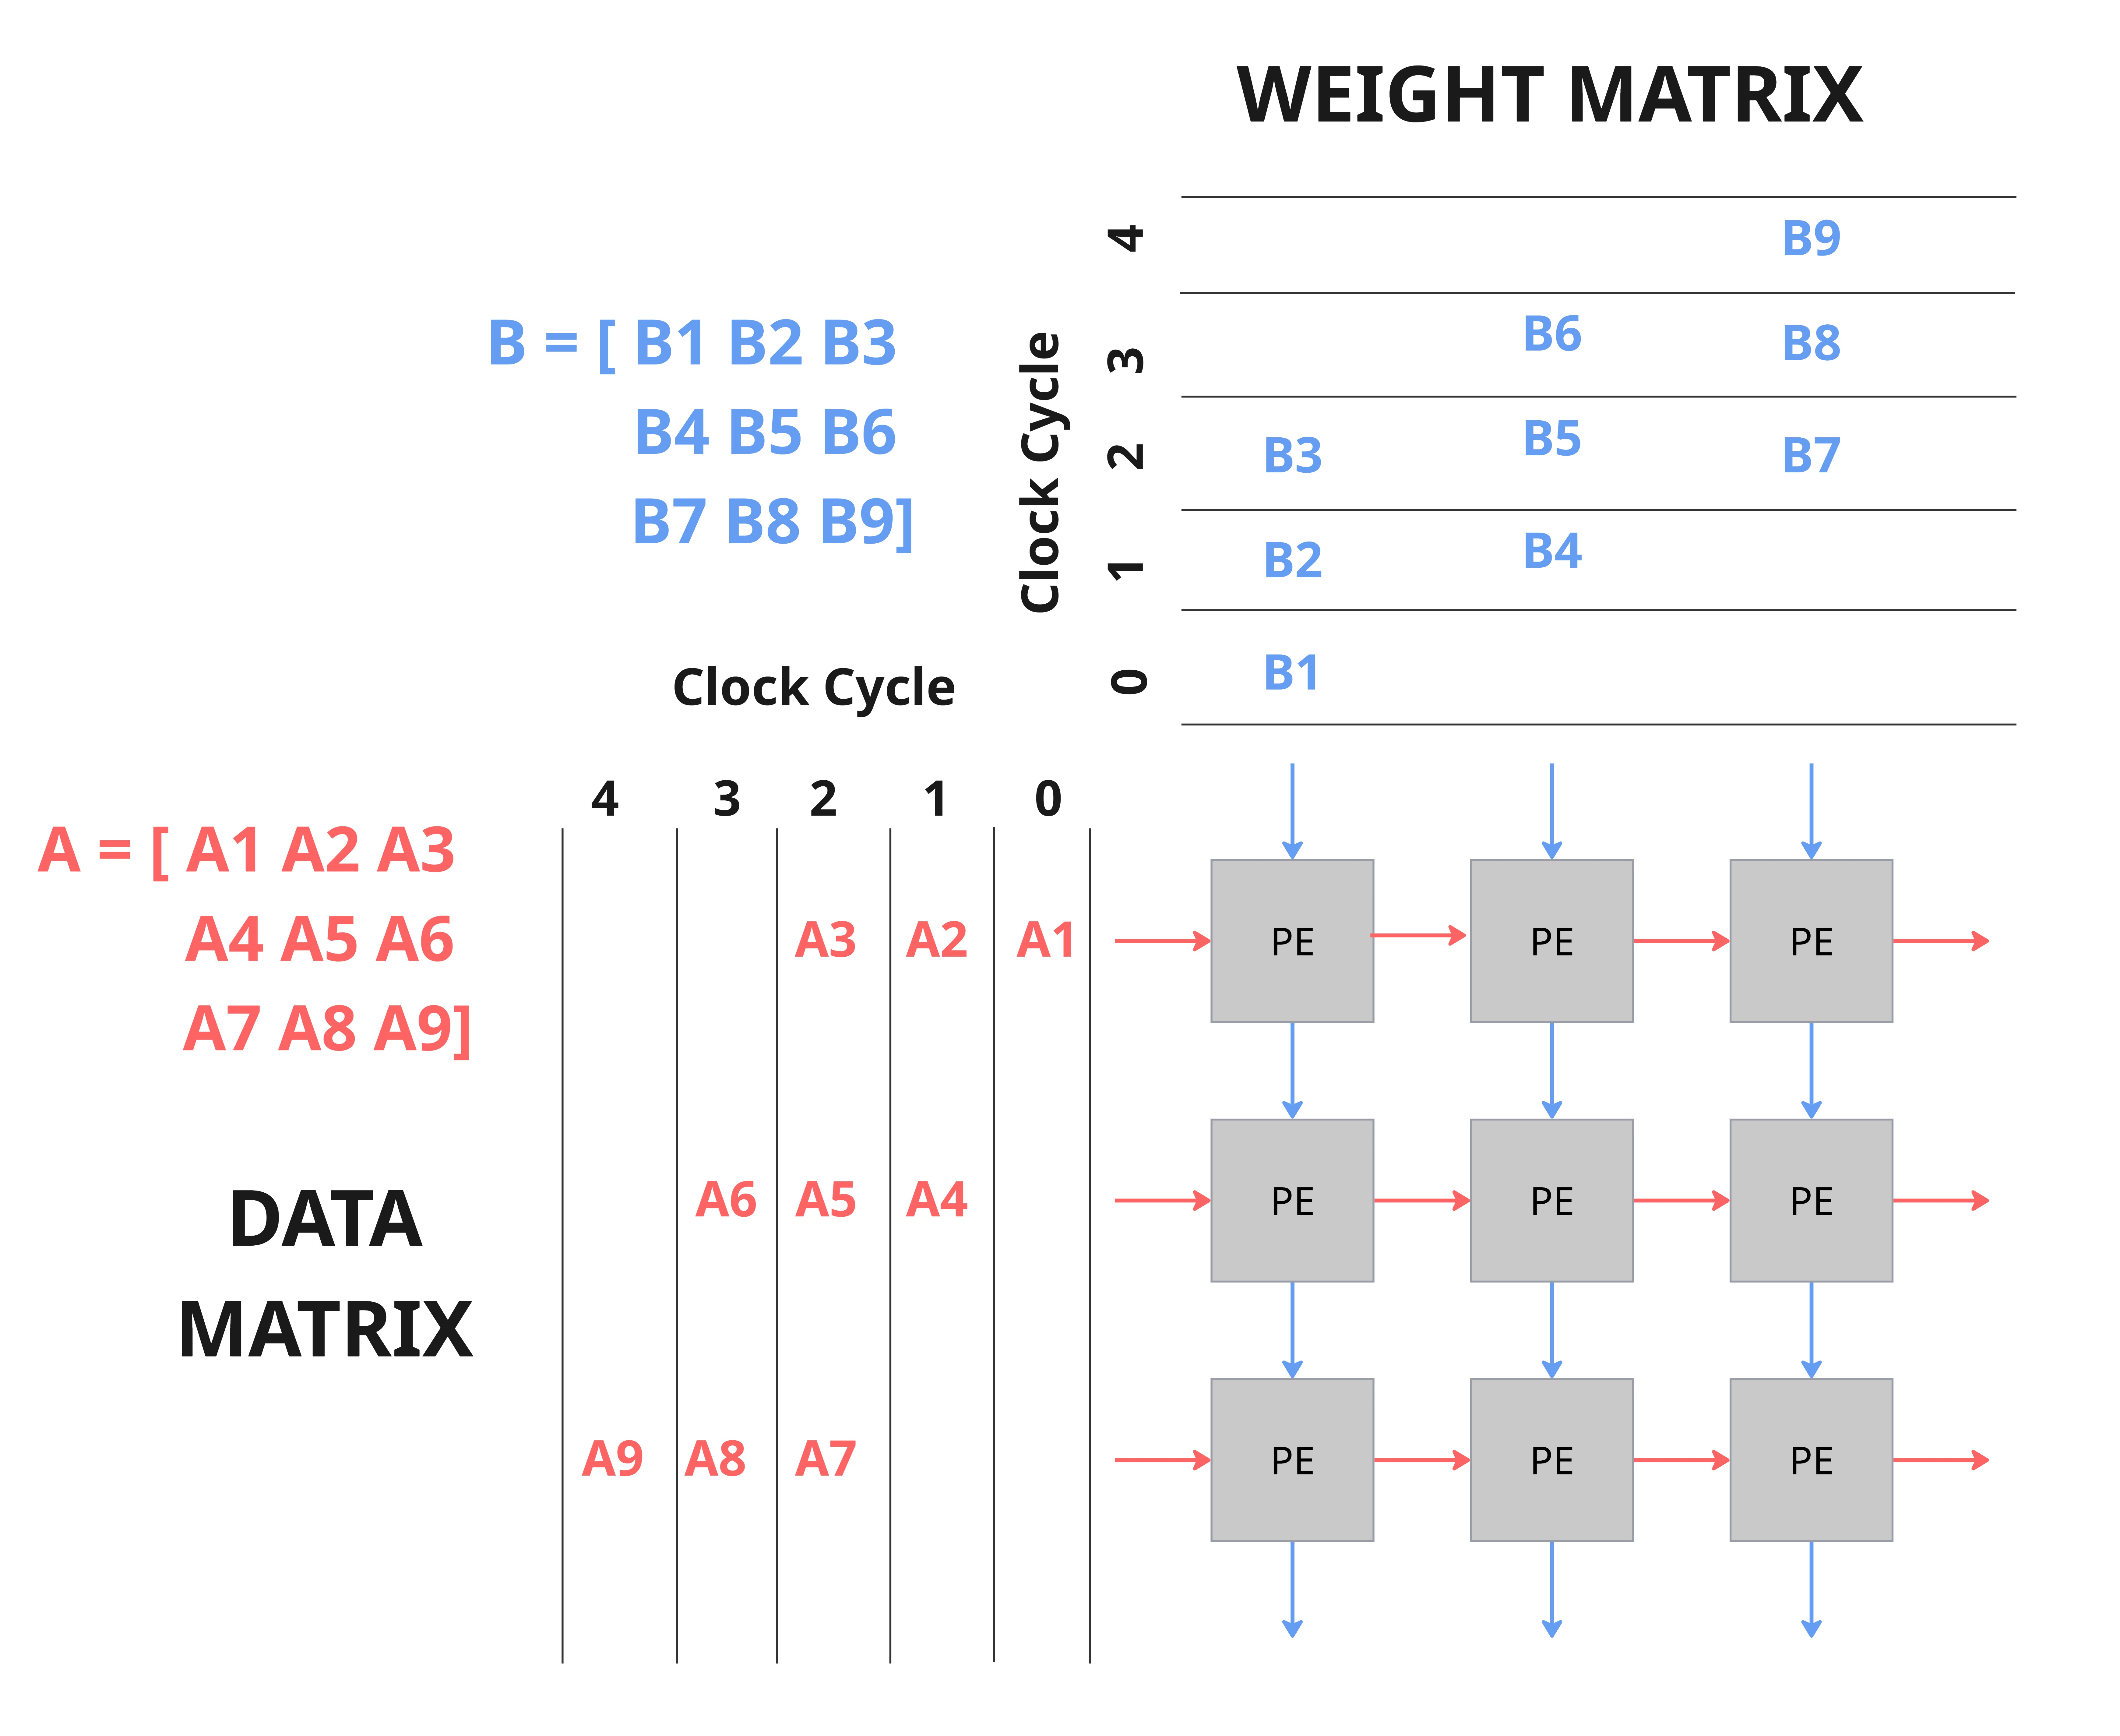
\includegraphics[width=0.5\linewidth]{figures/baseline_systolic_array_dataflow.jpg}
        \caption{Baseline Systolic Array's Dataflow}
        \label{fig:baseline_dataflow}
    \end{figure}
}

\newcommand{\performanceComparison}{
    \begin{figure}[ht]
        \centering
        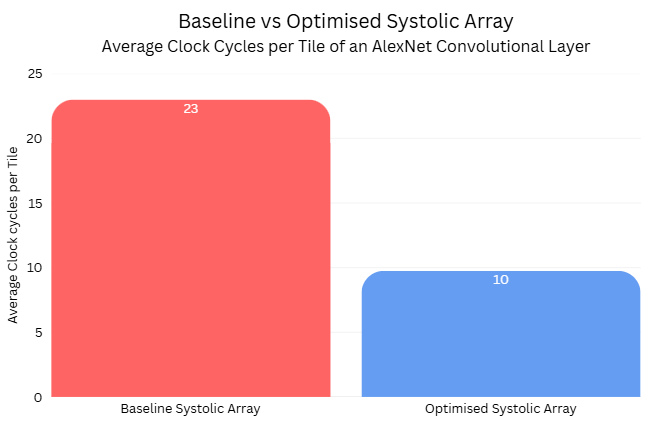
\includegraphics[width=0.5\linewidth]{results/Performance Comparison - Average Clock Cycles per Tile of an AlexNet Convolutional Layer.png}
        \caption{Performance Comparison: Average Clock Cycles per Tile of an AlexNet Convolutional Layer}
        \label{fig:performance_comparison}
    \end{figure}
}

\newcommand{\systemDiagram}{
    \begin{figure}[ht]
        \centering
        
\includegraphics[width=0.8\linewidth]{figures/system_diagram.jpg}
        \caption{System Overview of the Optimised Systolic Array, consisting of both Software and Hardware Components}  
        \label{fig:system_overview}
    \end{figure}
}

\newcommand{\RTL}{
    \begin{figure}[ht]
        \centering
        
\includegraphics[width=0.8\linewidth]{figures/rtl.jpg}
        \caption{Register Transfer Level (RTL) Diagram of the Processing Element (PE)}  
        \label{fig:rtl}
    \end{figure}
}

\newcommand{\tbFSM}{
    \begin{figure}[ht]
        \centering
        
\includegraphics[width=0.8\linewidth]{figures/tb_fsm.jpg}
        \caption{Testbench Finite State Machine (FSM) Diagram}
        \label{fig:tb_fsm}
    \end{figure}
}


%%%%%%%%%%%%%%%%%%%%%%%%%
% TABLES
%%%%%%%%%%%%%%%%%%%%%%%%%
\newcommand{\optimisedMValueFigure}{
    \begin{figure}[ht]
        \centering
        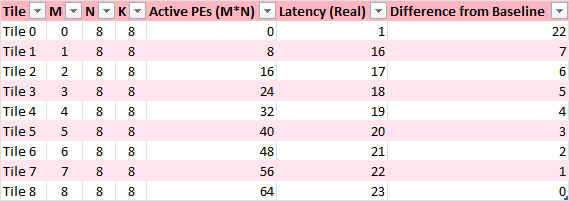
\includegraphics[width=0.5\linewidth]{results/Effect of M value on the number of Active PEs in the Systolic Array and Latency v2.png}
        \caption{Effect of M value on the number of Active PEs in the Systolic Array and Latency}
        \label{fig:optimised_m_value}
    \end{figure}
}



\newcommand{\optimisedLatencyRowStrippingFigure}{
    \begin{figure}[ht]
        \centering
        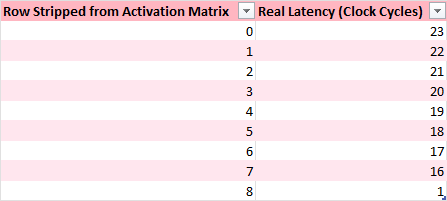
\includegraphics[width=0.2\linewidth]{results/Impact on Latency as Row Stripping Increases in a 8x8 Activation.png}
        \caption{Impact on Latency as Row Stripping Increases in a 8x8 Activation}
        \label{fig:latency_row_stripping}
    \end{figure}
}

\newcommand{\optimisedLatencyRowStrippingGraph}{
    \begin{figure}[ht]
        \centering
        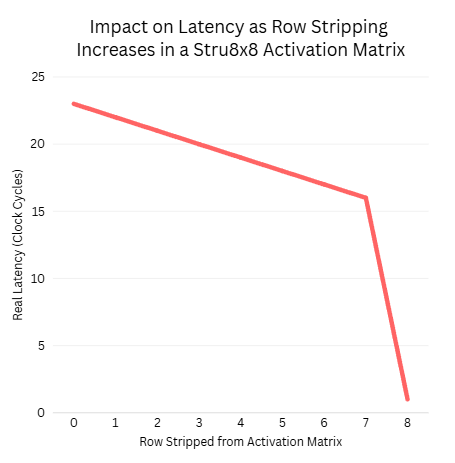
\includegraphics[width=0.4\linewidth]{results/Impact on Latency as Row Stripping Increases in a 8x8 Activation Graph.png}
        \caption{Impact on Latency as Row Stripping Increases in a 8x8 Activation}
        \label{fig:latency_row_stripping_graph}
    \end{figure}
}

\newcommand{\optimisedRandomSparsityGraph}{
    \begin{figure}[ht]
        \centering
        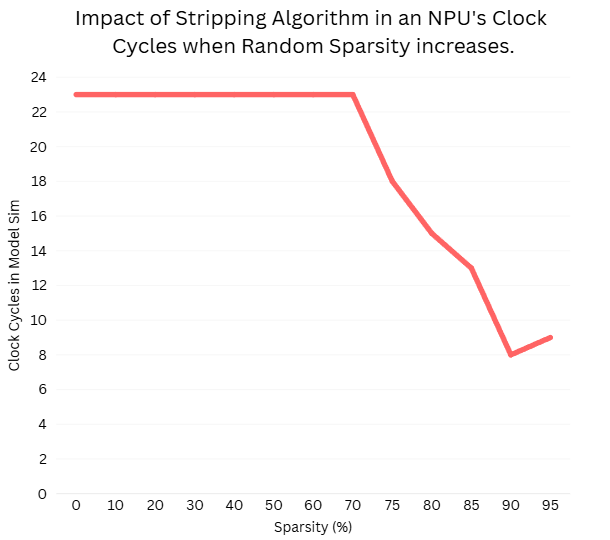
\includegraphics[width=0.4\linewidth]{results/Impact of Stripping Algorithm on Clock Cycles when Applied on Random Sparsity Graph.png}
        \caption{Impact of Stripping Algorithm on Clock Cycles when Applied on Random Sparsity}
        \label{fig:optimise_random_sparsity}
    \end{figure}
}

\newcommand{\fsmnpu}{
    \begin{figure}[ht]
        \centering
        
\includegraphics[width=0.8\linewidth]{figures/fsm_npu.jpg}
        \caption{Finite State Machine (FSM) Diagram of the NPU Loading Data from ROMs}
        \label{fig:fsmnpu}
    \end{figure}
}


\newcommand{\baselineNxN}{
    \begin{figure}[ht]
        \centering
        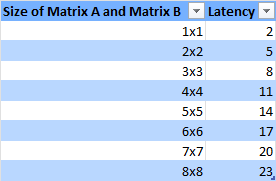
\includegraphics[width=0.3\linewidth]{results/Latency of Baseline Systolic Array on Different NxN sizes.png}
        \caption{Latency of Baseline Systolic Array on Different NxN sizes}
        \label{fig:latency_baseline_nxn}
    \end{figure}
}

\newcommand{\baselineNxEight}{
    \begin{figure}[ht]
        \centering
        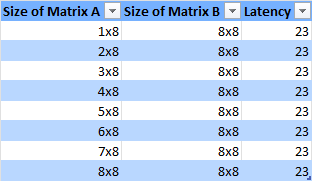
\includegraphics[width=0.3\linewidth]{results/Latency of Baseline Systolic Array on Varying Input Matrix Size.png}
        \caption{Latency of Baseline Systolic Array on Varying Input Matrix Size}
        \label{fig:latency_baseline_nxeight}
    \end{figure}
}


%%%%%%%%%%%%%%%%%%%%%%%%
%MODELSIM
%%%%%%%%%%%%%%%%%%%%%%%%
\newcommand{\baselineOnexOne}{
    \begin{figure}[ht]
        \centering
        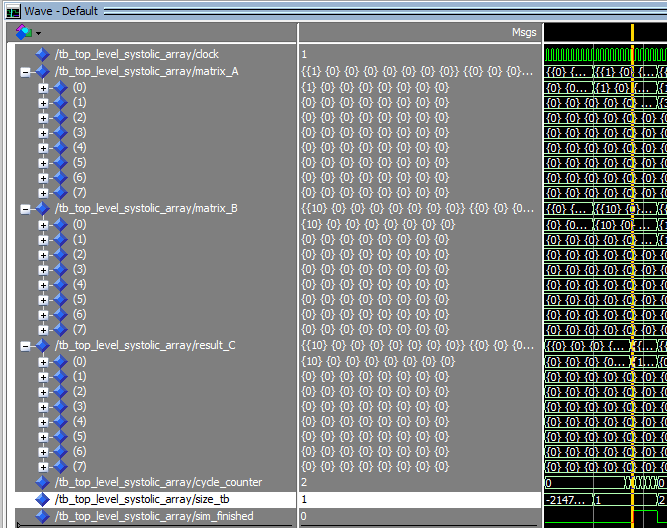
\includegraphics[width=0.2\linewidth]{results/baseline_modelsim/1x1.png}
        \caption{Latency of Baseline Systolic Array on 1x1 Input Matrix}
        \label{fig:latency_baseline_onexone}
    \end{figure}
}

\newcommand{\baselineOnexOneMATLAB}{
    \begin{figure}[ht]
        \centering
        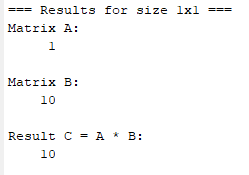
\includegraphics[width=0.2\linewidth]{results/baseline_modelsim/1x1_matlab.png}
        \caption{MATLAB Calculation of Baseline Systolic Array on 1x1 Input Matrix}
        \label{fig:latency_baseline_onexone_matlab}
    \end{figure}
}

\newcommand{\baselineTwoxTwo}{
    \begin{figure}[ht]
        \centering
        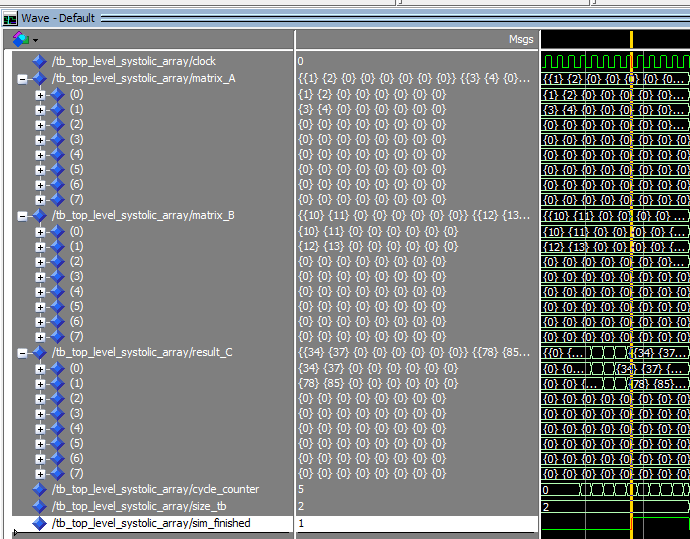
\includegraphics[width=0.2\linewidth]{results/baseline_modelsim/2x2.png}
        \caption{Latency of Baseline Systolic Array on 2x2 Input Matrix}
        \label{fig:latency_baseline_twoxtwo}
    \end{figure}
}

\newcommand{\baselineTwoxTwoMATLAB}{
    \begin{figure}[ht]
        \centering
        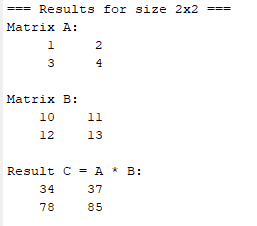
\includegraphics[width=0.2\linewidth]{results/baseline_modelsim/2x2_matlab.png}
        \caption{MATLAB Calculation of Baseline Systolic Array on 2x2 Input Matrix}
        \label{fig:latency_baseline_twoxtwo_matlab}
    \end{figure}
}

\newcommand{\baselineThreexThree}{
    \begin{figure}[ht]
        \centering
        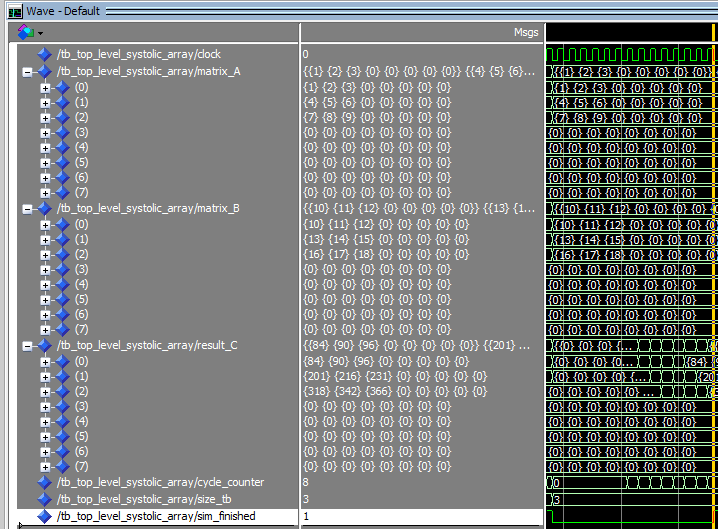
\includegraphics[width=0.2\linewidth]{results/baseline_modelsim/3x3.png}
        \caption{Latency of Baseline Systolic Array on 3x3 Input Matrix}
        \label{fig:latency_baseline_threexthree}
    \end{figure}
}
\newcommand{\baselineThreexThreeMATLAB}{
    \begin{figure}[ht]
        \centering
        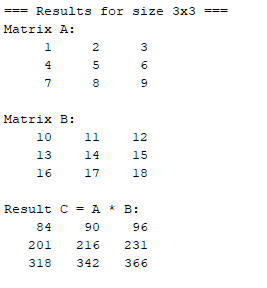
\includegraphics[width=0.2\linewidth]{results/baseline_modelsim/3x3_matlab.png}
        \caption{MATLAB Calculation of Baseline Systolic Array on 3x3 Input Matrix}
        \label{fig:latency_baseline_threexthree_matlab}
    \end{figure}
}

\newcommand{\baselineFourxFour}{
    \begin{figure}[ht]
        \centering
        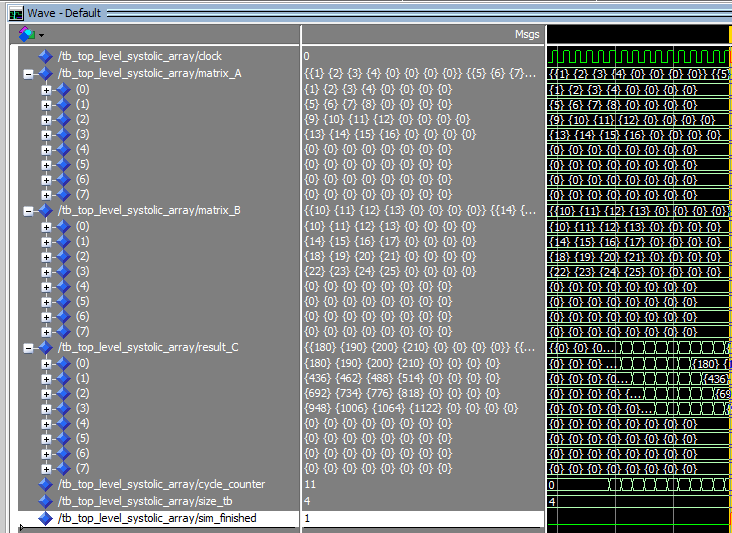
\includegraphics[width=0.2\linewidth]{results/baseline_modelsim/4x4.png}
        \caption{Latency of Baseline Systolic Array on 4x4 Input Matrix}
        \label{fig:latency_baseline_fourxfour}
    \end{figure}
}

\newcommand{\baselineFourxFourMATLAB}{
    \begin{figure}[ht]
        \centering
        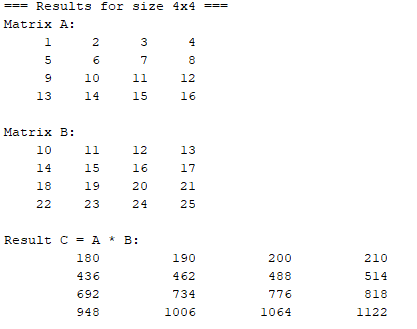
\includegraphics[width=0.2\linewidth]{results/baseline_modelsim/4x4_matlab.png}
        \caption{MATLAB Calculation of Baseline Systolic Array on 4x4 Input Matrix}
        \label{fig:latency_baseline_fourxfour_matlab}
    \end{figure}
}

\newcommand{\baselineFivexFive}{
    \begin{figure}[ht]
        \centering
        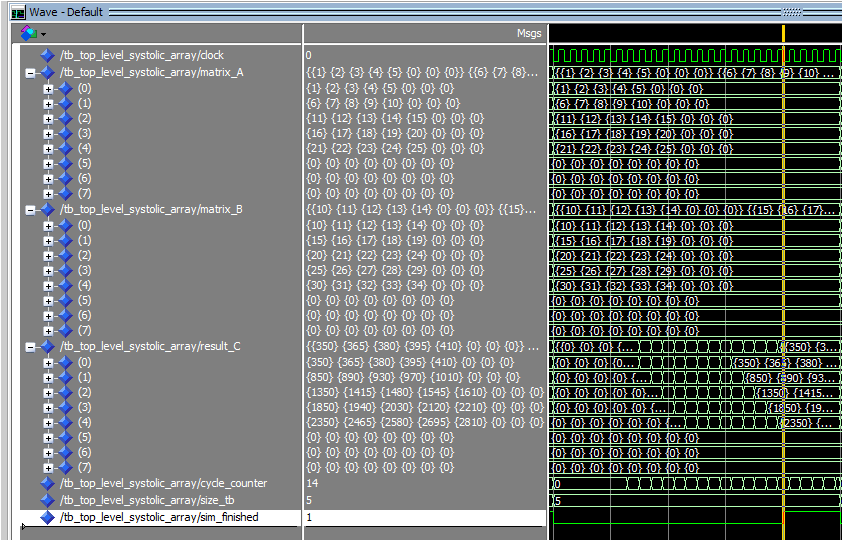
\includegraphics[width=0.2\linewidth]{results/baseline_modelsim/5x5.png}
        \caption{Latency of Baseline Systolic Array on 5x5 Input Matrix}
        \label{fig:latency_baseline_fivexfive}
    \end{figure}
}

\newcommand{\baselineFivexFiveMATLAB}{
    \begin{figure}[ht]
        \centering
        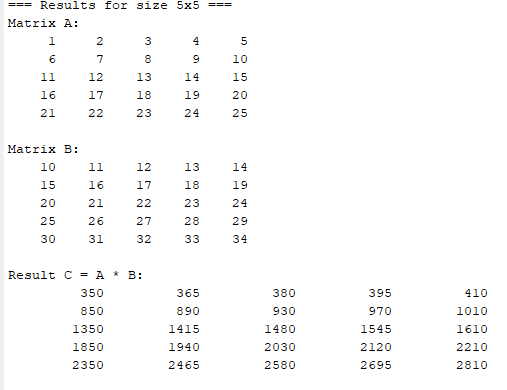
\includegraphics[width=0.2\linewidth]{results/baseline_modelsim/5x5_matlab.png}
        \caption{MATLAB Calculation of Baseline Systolic Array on 5x5 Input Matrix}
        \label{fig:latency_baseline_fivexfive_matlab}
    \end{figure}
}

\newcommand{\baselineSixxSix}{
    \begin{figure}[ht]
        \centering
        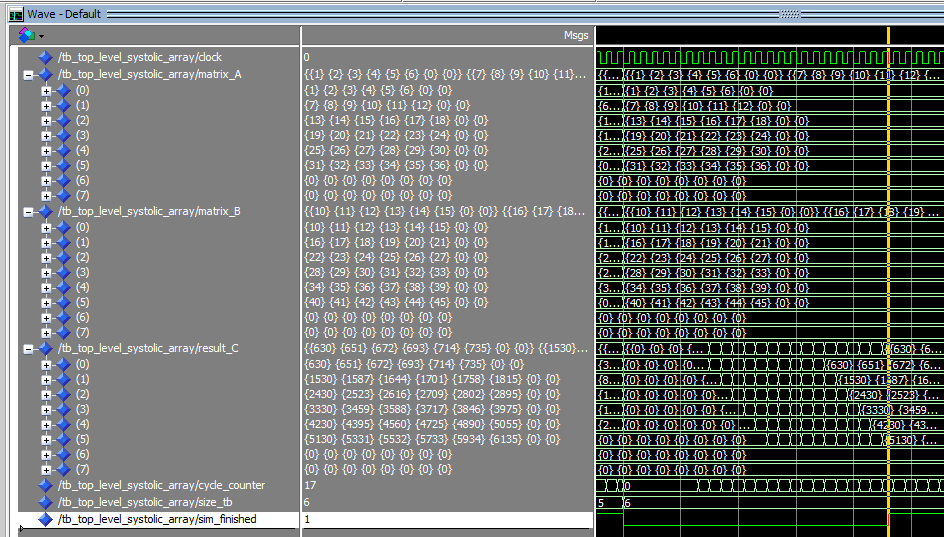
\includegraphics[width=0.2\linewidth]{results/baseline_modelsim/6x6.png}
        \caption{Latency of Baseline Systolic Array on 6x6 Input Matrix}
        \label{fig:latency_baseline_sixxsix}
    \end{figure}
}
\newcommand{\baselineSixxSixMATLAB}{
    \begin{figure}[ht]
        \centering
        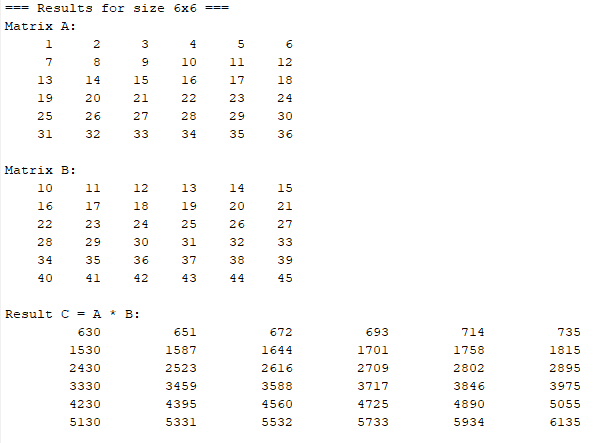
\includegraphics[width=0.2\linewidth]{results/baseline_modelsim/6x6_matlab.png}
        \caption{MATLAB Calculation of Baseline Systolic Array on 6x6 Input Matrix}
        \label{fig:latency_baseline_sixxsix_matlab}
    \end{figure}
}

\newcommand{\baselineSevenxSeven}{
    \begin{figure}[ht]
        \centering
        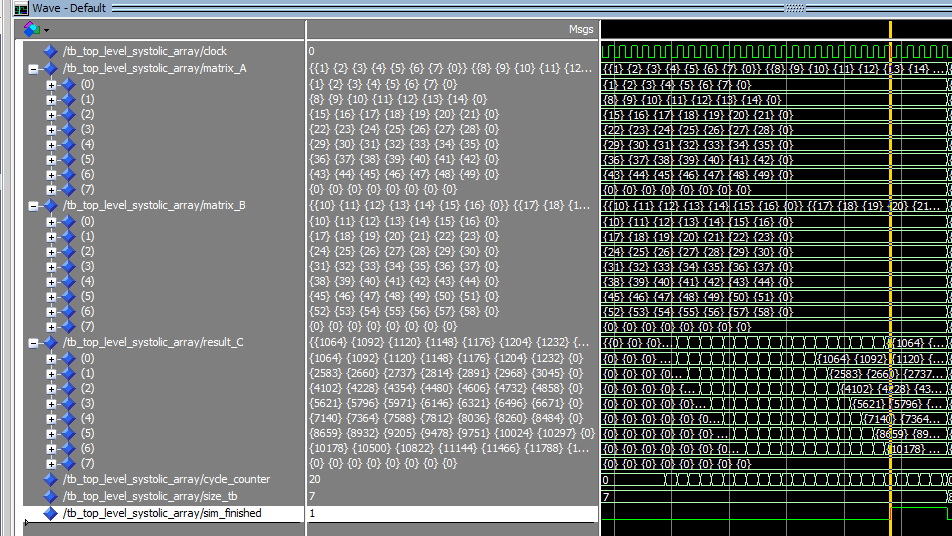
\includegraphics[width=0.2\linewidth]{results/baseline_modelsim/7x7.png}
        \caption{Latency of Baseline Systolic Array on 7x7 Input Matrix}
        \label{fig:latency_baseline_sevenxseven}
    \end{figure}
}
\newcommand{\baselineSevenxSevenMATLAB}{
    \begin{figure}[ht]
        \centering
        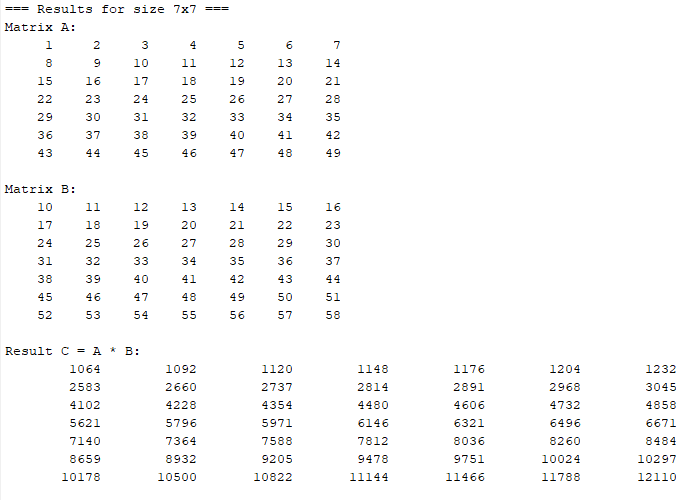
\includegraphics[width=0.2\linewidth]{results/baseline_modelsim/7x7_matlab.png}
        \caption{MATLAB Calculation of Baseline Systolic Array on 7x7 Input Matrix}
        \label{fig:latency_baseline_sevenxseven_matlab}
    \end{figure}
}

\newcommand{\baselineEightxEight}{
    \begin{figure}[ht]
        \centering
        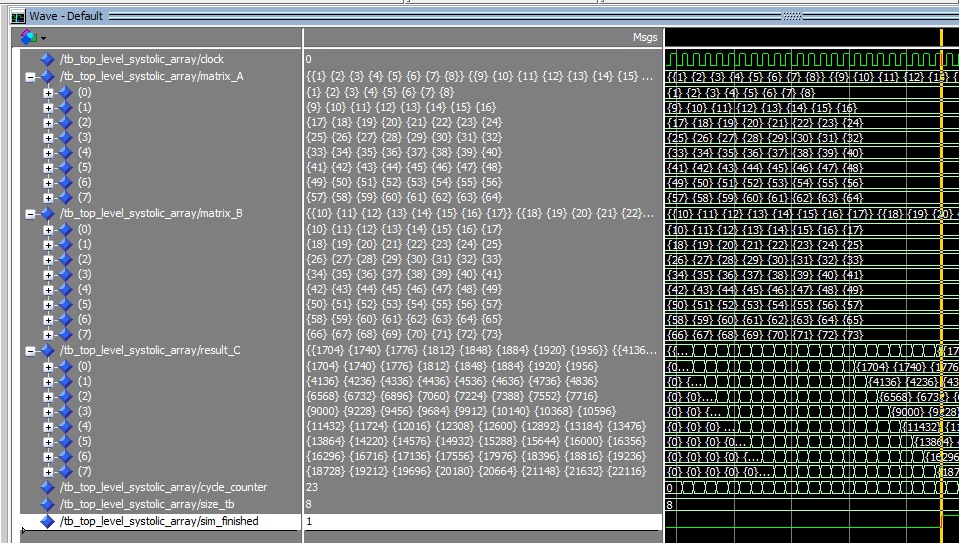
\includegraphics[width=0.2\linewidth]{results/baseline_modelsim/8x8.png}
        \caption{Latency of Baseline Systolic Array on 8x8 Input Matrix}
        \label{fig:latency_baseline_eightxeight}
    \end{figure}
}
\newcommand{\baselineEightxEightMATLAB}{
    \begin{figure}[ht]
        \centering
        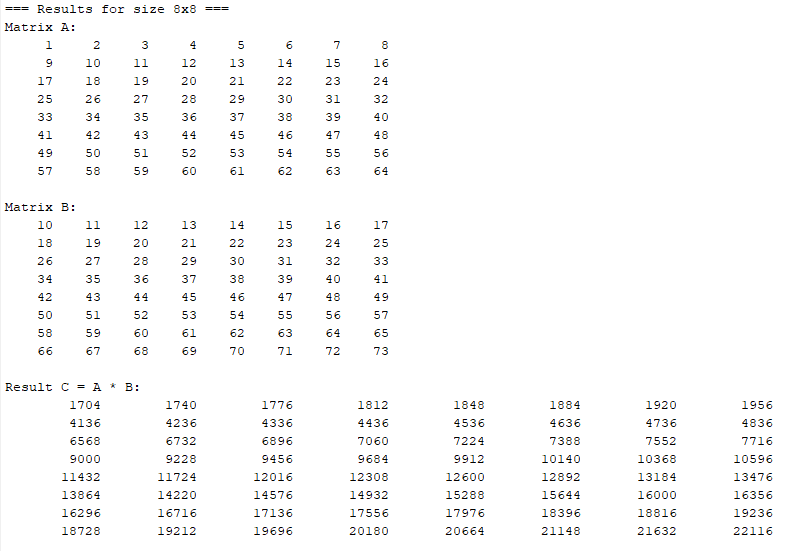
\includegraphics[width=0.2\linewidth]{results/baseline_modelsim/8x8_matlab.png}
        \caption{MATLAB Calculation of Baseline Systolic Array on 8x8 Input Matrix}
        \label{fig:latency_baseline_eightxeight_matlab}
    \end{figure}
}













% add page numbers
\fancyfoot[CO,CE]{\footnotesize\thepage}   % page number  
% line spacing 
\usepackage{setspace}
\setstretch{1.0}





%%%%%%%%%%%%%%%%%%%%%%%%%%%%%%%%%%%%%%%%%%%%%%%%%%%%%%%%%%%%%%%%%%%%%%%%%%%%%%%%
% DOCUMENT BODY
%%%%%%%%%%%%%%%%%%%%%%%%%%%%%%%%%%%%%%%%%%%%%%%%%%%%%%%%%%%%%%%%%%%%%%%%%%%%%%%%
\begin{document}
% 
% --- Define name and report number he
\def\name{Kristelle Sampang}
\def\reportNumber{COMPSYS043-\the\year}

% --- Title Page ---
\thispagestyle{empty}
\pagenumbering{roman}

\begin{center}
    \vspace*{10mm}
    % {\large \textbf{Research Project in Computer Systems Engineering}}

    \vspace*{10mm}
    \HRule
    
    \vspace{0.5cm}
    Final Report
    \vspace{0.5cm}
    
    {\Large \textbf{Project \#43: Reconfigurable Neural Processing Unit (NPU) for Energy-Efficient AI at the Edge}}
    
    \vspace{1cm}
    {\large \name}
    
    \vspace{0.5cm}
    Project Report 
    
    \vspace{0.5cm}
    \HRule
\end{center}

\vfill
\begin{center}
    \begin{tabular}{r l}
        \addlinespace[1.5em]
        Project Partner: & Pratham Chhabra \\
        \addlinespace[1.5em]
        Supervisor: & Dr Morteza Biglari-Abhari \\
        \addlinespace[1.5em]
        Co-Supervisor: & Dr Maryam Hemmati
    \end{tabular}
\end{center}

\vfill
\begin{center}
    \today
\end{center}

\vfill
\begin{center}
    % \includegraphics[width=0.7\linewidth]{figures/ecse-horizontal-hc.png}
    
\includegraphics[width=0.4\linewidth]{figures/UoA-Logo-Primary-RGB-Large.png}
\end{center}

\clearpage

% --- Abstract Page ---
\noindent \reportNumber

\vspace{1em}
\begin{center}
    {\large \textbf{\scshape Reconfigurable Neural Processing Unit (NPU) for Energy-Efficient AI at the Edge}}
\end{center}

\vspace{2em}
\begin{center}
    {\large \textbf{\name}}
\end{center}

\vspace{2em}
\begin{center}
    {\large \textbf{\scshape ABSTRACT}}
\end{center}

% Insert abstract here (approx. 250 words). The abstract should summarise the key points of the report, including the project objectives, methodology, results, and conclusions. It should be concise and informative, providing a clear overview of the report's content.


As Artificial Intelligence (AI) continues to rapidly advance, hardware accelerators, such as Neural Processing Units (NPUs), are becoming crucial in balancing high performance and energy-efficiency. The key motivator for this research is the growing demand for AI at the edge, where reduced power consumption and latency are essential considerations. One popular architecture for NPUs is the systolic array, efficient at parallelism for matrix multiplications commonly found in Convolutional Neural Networks (CNNs). However, the presence of sparsity in these networks, particularly due to ReLU activations, presents significant challenges to performance optimisation. Therefore, a software-hardware co-design approach is prposed to address this issue. A reconfigurable systolic array is implemented, capable of adpating to different levels of structured sparsity by implementing a row and column stripping algoirthm. This design is validated by synthesis on a DE1-Soc FPGA and by using a pre-trained AlexNet model on sample images, with performance compared against a baseline systolic array. The results demonstrate that the proposed approach significantly reduces latency compared to the baseline, with theoretical improvements of up to XX\% at higher sparsity levels. This research highlights the potential of reconfigurable NPUs in enhancing energy-efficient AI processing at the edge.



% --- Declaration Page ---
% \includepdf[pages=-, pagecommand={\thispagestyle{fancy}}]{Declaration.pdf}
\clearpage
\newpage
\vspace{2em}
\begin{center}
\Large\textbf{DECLARATION}
\end{center}
\noindent
\textbf{Student}
\vspace{1em}
I hereby declare that:
\begin{enumerate}
    \item This report is the result of the final year project work carried out by my project partner (see cover page) and I under the guidance of our supervisor (see cover page) in the 2025 academic year at the Department of Electrical, Computer and Software Engineering, Faculty of Engineering, University of Auckland. 
    \item This report is not the outcome of work done previously. 
    \item This report is not the outcome of work done in collaboration, except that with a potential project sponsor (if any) as stated in the text.
    \item This report is not the same as any report, thesis, conference article or journal paper, or any other publication or unpublished work in any format. 
\end{enumerate}
\vspace{1em}
\noindent
In the case of a continuing project, please state clearly what has been developed during the project and what was available from previous year(s): 
\vspace{3cm}
\noindent
\newline
Signature:

\includegraphics[width=0.3\linewidth]{figures/signature.png}

\vspace{1cm}
Date: 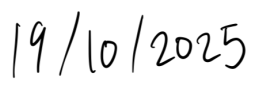
\includegraphics[width=0.2\linewidth]{figures/date.png}
% !! Remember to sign this

\newpage

% --- Table of Contents ---
\setlength{\parskip}{6pt}
\renewcommand{\contentsname}{\large{Table of Contents}}
\tableofcontents
\newpage
\setlength{\parskip}{9pt}

% --- Acknowledgements ---
\section*{Acknowledgements}
\addcontentsline{toc}{section}{Acknowledgements}

\label{sec:Acknowledgements1}
I would like to express my gratitude to my supervisors, Dr Morteza Biglari-Abhari and Dr Maryam Hemmati, for their guidance and support throughout this project. Without their assistance, this work would not have been possible. 
\newline \newline
I would like to extend my thanks to Pratham Chhabra, my project partner, for his hard work, collaboration, and dedication throughout this project. His efforts have been significant in the success of this work.

\newpage

% --- Glossary of Terms ---
\section*{Glossary of Terms}
\addcontentsline{toc}{section}{Glossary of Terms}

\begin{longtable}{p{0.25\linewidth} p{0.70\linewidth}}
    \toprule
    \textbf{Term} & \textbf{Definition} \\
    \midrule
    \endhead
    
    % 5G & Fifth generation mobile network \\

    AI at the Edge & Performing AI computations directly on edge devices rather than relying on cloud-based servers. \\
    
    Dataflow & The pattern of how data flows between processing elements and memory in a hardware accelerator. \\

    Hardware Acceleratgor & Specialised hardware designed to perform a particular task more efficiently than general-purpose processors. \\
    
    Latency & The time delay between the input and output of a system, measured in clock cycles for this project. \\
  
    Pruning & Technique to remove unnecessary weights in a neural network to compress the model. \\ 
  
    Quantisation & Reducing the precision of numbers to make the model smaller and faster. \\
  
    Sparsity & The presence of a significant number of zero-valued elements in a matrix or tensor. \\

    Systolic Array & Network of processing elements that rhythmically compute and pass data through the system. \\
    
    Tiling & Breaking large matrices into smaller, fixed-sized blocks to fit into hardware constraints. \\ 
    \bottomrule
\end{longtable}
\addtocounter{table}{-1}

% --- Abbreviations ---
\section*{Abbreviations}
\addcontentsline{toc}{section}{Abbreviations}

\begin{longtable}{p{0.25\linewidth} p{0.70\linewidth}}
    \toprule
    \textbf{AOA} & \textbf{Angle of attack} \\
    \midrule
    \endhead
    AI & Artificial Intelligence \\
    CNN & Convolutional Neural Network \\
    CPU & Central Processing Unit \\
    DNN & Deep Neural Network \\
    DPR & Dynamic Partial Reconfiguration \\
    FPGA & Field-Programmable Gate Array \\
    FSM & Finite State Machine \\ 
    GPU & Graphics Processing Unit \\
    MAC & Multiply-Accumulate \\
    MIF & Memory Initialization File \\
    ML & Machine Learning \\
    NPU & Neural Processing Unit \\
    PE & Processing Element \\
    ReLU & Rectified Linear Unit \\
    ROM & Read-Only Memory \\
    RTL & Register-Transfer Level \\

    \bottomrule
\end{longtable}
\addtocounter{table}{-1}

% --- Nomenclature ---
\printnomenclature

\clearpage
\setlength{\parskip}{9pt}
\pagenumbering{arabic}
% --- Main Body of the Report ---
\section{Introduction} \label{sec: intro}
    % \subsection{Motivation}
    % Hook the reader. Why is this project important? What is the big-picture problem? 
    % (e.g., The explosion of AI and IoT devices demands powerful but low-power processing directly on the edge.)
    % Why are current solutions like CPUs/GPUs not good enough for this specific problem? (e.g., Power consumption, size constraints.)

    % \begin{itemize}
    %     \item As the demand for artificial intelligence grows to become prominent in today's society, its energy consumption has become a key issue. 
    %     \item The processing required to run machine learning models is large, with millions of computations needed to be executed. 
    %     \item This means that low-power processing devices at edge are limited to its use. 
    %     \item The processing power to run machine learning models is large, limiting its use for low-power processing devices at the edge.  
    %     \item With high computational power required, energy-efficiency is a key concern, especially nowadays when energy is an essential resource to not waste.
    %     \item In the past decade, common types of processors for running AI are CPU, GPU, and FPGA. 
    %     \item However, as technology continues to improve, Neural Processing Units (NPU) are developed. These are processors that specialise in processing AI computations.
    %     \item By integrating NPU alongside other processors, the performance and energy-efficiency are improved compared to a standalone processor. 
    %     % \item This report aims to focus on tacking the issue of low energy-efficient use of AI at edge. 
    %     %% I need more context here
    % \end{itemize}
    The demand for Artificial Intelligence (AI) has grown exponentially in recent years, becoming prominent in various aspects of today's society. However, the energy consumption associated with AI has emerged as a critical concern. The execution of Machine Learning (ML) models requires a considerable amount of processing power, involving millions of computations. This high computational demand presents a limitation for low-power processing devices, particularly those operating at the edge. As technology continues to evolve, specialised processors, such as Neural Processing Units (NPU), have been developed to address the specific needs of AI computation. 

    These NPUs are specialised to execute algorithms more efficiently than general-purpose CPUs and GPUs, offering significant improvements in both performance and energy efficiency. A common architecture for NPUs is the systolic array, which allows for parallel processing of data, thereby reducing latency and power consumption. This architecture is perfect for the common computation found in Convolutional Neural Networks (CNNs), which rely heavily on matrix multiplications. However, this architecture is challenged by the presence of sparsity in these networks. Therefore, addressing the issue of sparsity is crucial for optimising the performance of NPUs in real-world applications.

    This project aims to design and implement a reconfigurable Neural Processing Unit (NPU) that optimises energy efficiency for AI applications at the edge. The specific objectives of this project are as follows:
    \begin{itemize}
        \item Design a reconfigurable NPU architecture that can adapt to varying computational requirements of different AI models.
        \item Implement energy-efficient dataflow strategies to minimise power consumption during AI inference tasks.
        \item Evaluate the performance and energy efficiency of the proposed NPU design through simulations and benchmarking against existing solutions.
        \item Develop a software-hardware co-design approach to facilitate the integration of the NPU with existing AI frameworks.
        \item Demonstrate the effectiveness of the NPU in real-world edge computing scenarios.
    \end{itemize}



    The remainder of this report is organised as follows: Section~\ref{sec: background} provides the necessary background on the core ideas that support this project, including Convolutional Neural Networks (CNNs) and hardware acceleration for machine learning. Section~\ref{sec: literature review} reviews existing literature and related work in the field, highlighting the gaps that this project aims to address. Section~\ref{sec: design_method} details the methodology employed in designing and implementing the reconfigurable NPU. Section~\ref{sec: verification} verifies the proposed design and presents the results obtained from simulations. Section~\ref{sec: discussion} discusses the implications of the results, comparing them with existing solutions and outlining potential areas for improvement. Finally, Section~\ref{sec: conclusion} concludes the report by summarising the key findings and and Section \ref{sec: future work} discusses potential future work.

\clearpage  
\newpage
\section{Background} \label{sec: background}
    % According to the rubric, this section must "Clearly define the project context" and demonstrate
    % "a good understanding of the broader scientific or engineering domain."
    % Think of this section as bringing a reader up to speed on the core technologies you're using.
    The increasingly growth of Artificial Intelligence (AI) in the past decade has driven significant advancements across numerous field. Machine Learning (ML) models, particularly Deep Neural Networks (DNNs), are popular for its applications from image classification to autonomous driving \cite{parashar_scnn_2017}. There has been significant shift from AI inferencing occurring at a cloud-level to resource-constrained edge devices. This move motivates the \textit{AI at the Edge} portion in the research, where lower latency, enhanced data privacy, and real-time processing capabilities must are requirements that must be met without relying on constant network connection \cite{kim_energy-efficient_2020}.

    However, this shift presents an alarming issue where DNNs are computationally intensive and power-hungry, whilst edge devices operate under strict power and resource limitations. To bridge this gap, hardware accelerators, such as Neural Processing Units (NPUs), are introduced to execute AI algorithms at faster rates than general-purpose CPUs \cite{manor_custom_2022}. This section provides necessary background on the core technologies that support this project, starting with the most popular model for image-based tasks: the Convolutional Neural Network.

    \subsection{Convolutional Neural Networks (CNN)} \label{sec:CNN}
    Convolutional Neural Networks (CNNs) are a prominent type of DNN~model, mainly utilised for image processing tasks like object recognition, classification, and detection. The network is composed of four main layers: convolutional, activation, pooling, and fully connected layers; this research focuses on the convolutional and activation layers. The convolutional layer is where the majority of the computations occur \cite{choi_enabling_2023}, as it extracts features from an image and converts them into numerical values. In a convolutional layer, there are several filters that slide through the image, searching for a specific pattern. These filters are typically of size $3\times3$ or $5\times5$, and are applied to the image by multiplying the filter by the 2D pixel representation of the image. Mathematically, this operation can be represented as:
    \[
    O[h][w][c] = \sum_{i=1}^{f_h} \sum_{j=1}^{f_w} \sum_{k=1}^{i_c} I[h + i \cdot s_h][w + j \cdot s_w][k] \times F[i][j][k][c]
    \]

    where I, O, F are input activation, output activation, and filter weights respectively \cite{choi_enabling_2023}. This can be represented as an enormous number of Multiply-Accumulate (MAC) operations, making CNNs computationally intensive. 

    An activation layer determines whether a neuron should be activated based on its input. Its primary role is to introduce non-linearity into the network. Without this, a neural network can only learn simple, linear patterns. Non-linearity allows the network to execute complex tasks, such as learning complicated patterns. A commonly used function is the Rectified Linear Unit (ReLU). The main functionality is to allow for positive inputs to remain unchanged whist setting any negative input to zero \cite{parashar_scnn_2017}. Mathematically, this can be represented as:
    \[
    \text{ReLU}(x) = 
    \begin{cases} 
        1 & \text{if } x > 0 \\ 
        0 & \text{if } x \le 0 
    \end{cases}
    \]



    A critical consequence of this is that it introduces significant sparsity as approximately half of the elements are zero~\cite{sun_sense_2023}. This sparsity is a key property that this project exploits to improve energy-efficiency, and will be discussed further in Section~\ref{sec:relu}.

    Although not the core focus of this project, the pooling layers are used to reduce the spatial dimensions of the input whilst retaining the most relevant features. This helps to decrease computational load and control overfitting. Furthermore, a fully connected layer is typically used at the end of the CNN to perform high-level reasoning based on the features extracted by previous layers\cite{cain_convolution_2021}.




    \subsection{Hardware Acceleration for Machine Learning} \label{sec: hardware accel}
    % A study discovered that GPUs highly accelerate computationally intensive tasks with parallelism at ease but with a trade-off of high power consumption \cite{oh_investigation_2017}. Furthermore, GPUs are not typically found in edge devices, such as smartphones and IoT devices, due to its high power consumption and thermal output. Conversely, Neural Processing Units (NPUs) are a type of specialised hardware accelerator, best a executing AI-based algorithms. Due to its dedicated use, it has extreme performance and low-energy effiency, however, it is limited in its flexibility. Alternatievvly, FPGAs can achieve energy-efficiency by consuming half the power of a GPU\cite{liu_energy-efficient_2024} by tailoring the hardware architecture to a specific task. This customisability allows for optimised dataflow and memory access patterns, crucial for improving the performance of deep learning models. Therefore, this project chooses to implement the NPU on an FPGA platform to create a reconfigurable hardware accelerator.
    General-purpose CPUs alone are not powerful enough to handle the computational requirements of modern deep learning models \cite{zhang_energy-efficient_2022}. This puts additionally strain on edge devices, which are typically resource-constrained and have limited power budgets. This means that specialised hardware accelerators are needed to efficiently execute AI algorithms \cite{manor_custom_2022}. Typically, multiple processes exist in parallel, such as Graphical Processing Units (GPUs), Field Programmable Gate Arrays (FPGAs), and Neural Processing Units (NPUs), and are integrated with the CPU as a heterogeneous system  to enhance the performance of AI applications \cite{manor_custom_2022}. Several studies have compared these hardware accelerators for AI applications, summarised as follows:
    \begin{itemize}
        \item A study discovered that \textbf{GPUs} highly accelerate computationally intensive tasks with parallelism at ease but with a trade-off of high power consumption \cite{oh_investigation_2017}. Furthermore, GPUs are not typically found in edge devices, such as smartphones and IoT devices, due to its high power consumption and thermal output. 
        \item \textbf{NPUs} are a type of specialised hardware accelerator, best at executing AI-based algorithms. Due to its dedicated use, it has extreme performance and low-energy efficiency, however, it is limited in its flexibility.
        \item \textbf{FPGAs} can achieve energy-efficiency by consuming half the power of a GPU \cite{liu_energy-efficient_2024} by tailoring the hardware architecture to a specific task. 
    \end{itemize}
    
    The customisability of FPGAs allows for optimised dataflow and memory access patterns, crucial for improving the performance of deep learning models. This provides a platform to design and implement specialised NPUs that can efficiently handle the unique demands of AI workloads. Therefore, this project chooses to implement the NPU on an FPGA to create a reconfigurable hardware accelerator. 

    


    
    % \cite{manor_custom_2022}: why we are making a hardware accelerator "However, the high computational demand required for Machine Learning (ML) inference on tiny microcontroller-based IoT devices avoids a direct software deployment on such resource-constrained edge devices. Therefore, various custom and application-specific NN hardware accelerators have been proposed to enable real-time Machine Learning (ML) inference on low-power and resource-limited edge devices." 
    % \cite{liu_energy-efficient_2024}: based on the table, we see that the CPU/FPGA relationship tends to perform best at image processing tasks


    \subsection{Systolic Array Architecture} \label{sec: systolic array }
    % A systolic array is a structured network of processing elements (PEs) where computations are carried out in a systematic approach, similar to pipelining \cite{kung_systolic_1978}. Each PE will receive, process, and pass on data to its neighbour concurrently in one clock cycle. Due to this, it provides characteristics like parallel computing, pipelining, synchronicity, and spatial and temporal locality.  These are advantageous as processes are completed simultaneously at higher speeds, computations are timed by a global clock for predictable data movement, and faster memory accessing time. Additionally, systolic arrays are highly compact together and allow simple data control flow. As its architecture is an array, it can easily be scaled for larger data sets, perfect for ML, and the predictable structure makes it easier to design and optimise algorithms. Furthermore, since the PEs are densely packed together, there are less data transmission, causing lower energy consumption. Energy-efficiency is a critical consideration when designing hardware accelerators for edge devices, where power resources are limited. Efficient energy usage not only extends battery life but produces less heat, important for maintaining device performance and lifespan. 
    % \newline 
    % However, there are some disadvantages to systolic arrays. These include difficult and costly to build and specialised and inflexible in the problems it can solve, limiting its versatility. Because systolic arrays offer high throughput and efficiency, it is commonly used in NPUs to accelerate matrix multiplication, the core operation in a CNN's convolutional layer. However, its rigid and structured dataflow is inefficient for sparse matrices, leading to imbalanced workloads and low PE utilisation. This limitation motivates the need for a reconfigurable systolic array that can adapt to the sparsity in neural networks, becoming the focus of this project.
    A systolic array is a structured network of interconnected processors known as Processing Elements (PE) that perform computations in a rhythmic and synchronised manner \cite{kung_systolic_1978}. Each PE receives data, processes it, and passes it to the next PE in a pipelined fashion \cite{sun_sense_2023}, allowing for high levels of parallelism and efficient data flow. This structure allows processes to be completed at higher speeds, with computations timed by a global clock for predictable data movement and faster memory access times. Additionally, systolic arrays are highly compact together and allow simple data control flow. As its architecture is an array, it can easily be scaled for larger data sets, perfect for ML, and the predictable structure makes it easier to design and optimise algorithms. Furthermore, since PEs are densely packed together, data locality is improved, reducing data transmission and lowering energy consumption. Energy-efficiency is a critical consideration when designing hardware accelerators for edge devices, where power resources are limited. Efficient energy usage not only extends battery life but produces less heat, important for maintaining device performance and lifespan. .
    \newline \newline
    Although it offers many advantages, there are some disadvantages to systolic arrays. These include being difficult and costly to build, as well as being specialized and inflexible in the problems it can solve, limiting its versatility. Because systolic arrays offer high throughput and efficiency, it is commonly used in NPUs to accelerate matrix multiplication \cite{seo_versa_2024}, the core operation in a CNN's convolutional layer. However, its rigid and structured dataflow is inefficient for sparse matrices \cite{he_sparse-tpu_2020,sun_sense_2023}, leading to imbalanced workloads and low PE utilisation. This limitation motivates the need for a reconfigurable systolic array that can adapt to the sparsity in neural networks, becoming the focus of this project.
    
    

    % !! insert image from that paper for visuals

    % - As systolic arrays offer high throughput, this suggests that it can help improve upon energy-efficiency when processing neural networks. 

    
    % Energy-efficiency is a critical consideration in the design of hardware accelerators for AI, especially for edge devices where power resources are limited. Efficient energy usage not only extends battery life but also reduces heat generation, which is vital for maintaining device performance and longevity. Techniques such as quantisation and pruning are commonly employed to enhance energy-efficiency in neural networks. Quantisation reduces the precision of the weights and activations, leading to lower computational requirements and reduced memory bandwidth. Pruning, on the other hand, eliminates redundant or less significant weights, resulting in sparser models that require fewer computations. Both techniques contribute to reducing the overall energy consumption of AI models without significantly compromising their performance. This project aims to leverage these energy-efficient techniques within a reconfigurable systolic array architecture to optimize the processing of sparse neural networks, thereby addressing the challenges associated with energy consumption in edge AI applications.


    % !! energy-efficiency section from original literature review (quantisation, pruning etc)
    % !! motivation for energy efficiency 
    % !! tie in everything together to motivate the project and bridge it with the rest of the literature review 


% --- Literature Review ---
\section{Literature Review} \label{sec: literature review}


    This section delves deep into the novelties and gaps in the current research on handling sparsity in neural networks, particularly in the context of systolic arrays. It explores the challenges posed by sparsity and reviews existing hardware architectures designed to mitigate these issues, leading to the motivation for this project.   


    \subsection{Sparsity in Neural Networks} \label{sec: sparsity in nn}
    % Explain where the zeros come from and why they are a problem.
    % 1.  **Introduce Sparsity**: Define sparsity as the presence of a large number of zero values in
    %     the weight and activation matrices.
    % 2.  **Sources of Sparsity**:
    As discussed in Section \ref{sec:CNN}, sparsity is a property of matrices that arise from many sources, such as activation functions and model compression techniques. This section explores these in detail to find the root cause of sparsity in neural networks. 

        \subsubsection{Rectified Linear Unit (ReLU)} \label{sec:relu}
        To optimise the performance of a neural network, gradients are calculated to update the network's weights. However, this introduces the Vanishing Gradient Problem (VGP) where gradients become increasingly miniscule when backpropagated from the output to earlier layers \cite{tan_vanishing_2019}. The consequence of VGP presents slow convergence and impaired learning. This issue becomes even more problematic when structures have many layers and a solution to this is applying ReLU. As previously mentioned in Section \ref{sec:CNN}, the outcome of ReLU is that all negative values are set to zero, introducing significant sparsity in the activation matrices. However, since ReLU is most commonly applied \cite{sun_sense_2023}, it is difficult to avoid using a model that does not produce sparse matrices due to ReLU in real-case scenarios.


    
        \subsubsection{Pruning}\label{sec:pruning}

    Model Pruning is a technique used to remove redundant data that may not significantly contribute to the final prediction. \textcite{kim_fpga_2021} found that more than half of weights in convolutional layers can be set to zero without impacting the overall accuracy. To decide what weights to prune, the sensitivity of the weight is considered and how it influences the output. \textcite{gorvadiya_energy_2025} discovered that their Weight Pruning technique resulted in minimal accuracy loss of 1-2\% whilst saving 25\% in power consumption. These results suggests that pruning is an effective method to reduce model size and computation without sacrificing performance.

    Whilst both ReLU and pruning work together to help accelerate the efficiency of the neural network by introducing sparsity in the system, this presents a challenge for systolic array based hardware architecture.
    As the architecture of systolic arrays is rigid and structured, it is advantageous for dense matrices with regular data access patterns. However, with the introduction of irregularity due to sparsity, this leads to inefficient memory access patterns and imbalanced workloads, causing low PE utilisation \cite{he_sparse-tpu_2020}. Additionally, with the high volume of computations required to run a CNN, the impact of the inefficiency is magnified. This means that handling sparsity is a critical issue that must be solved to fully exploit the benefits of sparsity in neural networks. Balancing the benefits and drawbacks of how sparsity is handled in systolic arrays is explored in the following section.

    \subsection{Hardware Architectures for Sparsity} \label{sec: hardware arch spars}
    % Now, review what others have done to solve the sparsity problem.
    % !! introductory / bridging paragraph
    This section explores various hardware techniques that have been discovered to handle sparsity in neural networks. The main methods are power-gating and zero-skipping, compressed data formats, and specialised dataflows and architectures. Each method has its own advantages and disadvantages, discussed in detail below.
        \subsubsection{Power Gating and Zero-Skipping} \label{sec: power-gating}
        As multiplying and accumulating with zero does not change the overall result, it is redundant to execute operations with zero. Thus, a method like power-gating is introduced to skip these unnecessary operations. The most straight forward approach to handling sparsity in hardware is power-gating. This method skips the MAC operation if one of the operands is zero, dynamically saving power \cite{parashar_scnn_2017}. However, this method requires additional hardware to check if an operand is zero, adding complexity to the design. Additionally, this does not reduce the latency as the PE has to wait for the data to be fetched from memory for the systolic pipeline to advance at the same rate.
        
        A more advanced approach that reduces latency is zero-skipping. This technique involves only processing non-zero values and skipping over the zeros entirely. On a smaller scale, this can be applied to individiual weights to reduce the number of clock cycles \cite{duk_kim_24_2020}. On a larger scale, in the architecture by \textcite{kim_fpga_2021}, the accelerator was able to skip 128x128 square blocks if structured sparsity existed, leading to a significant reduction in latency. However, this requires high levels of structured sparsity, that may not always occur in real-case scenarios.

        \subsubsection{Compressed Data Formats} \label{sec: compressed}
        To further improve performance, many architectures use compressed data formats to reduce the significant energy and latency costs of memory access. This is often implemented as a software-hardware co-design where a pre-processing stage reorganises the sparse matrix before it is sent to the accelerator. For example, \textcite{he_sparse-tpu_2020} proposes a packing technique to confense the matrix offline then loads it into the systolic array. Similarly, \textcite{seo_versa_2024} uses a pre-processing column-wise condensation of the weights to remove zero values in advanced. Additionally, \textcite{palacios_systolic_2025,kim_fpga_2021} found that with structured pruning, where entire rows or columns of weights are pruned, the hardware can be optimised to skip entire rows or columns of computations. This is more efficient than unstructured pruning, where individual weights are pruned, as it maintains the regularity of the data access patterns. 

        Although these methods significantly reduce memory access costs and improve performance, there are trade-offs. As these methods change the structure of the input matrices, it requires complex hardware and control logic to manage the new dataflow. Additionally, post-processing is required to rearrange the result matrix is required to ensure that the indices match up the original input \textcite{seo_versa_2024}. This added complexity may lead to increased power consumption and use of hardware resources, potentially nullifying the benefits of handling sparsity. Therefore, whilst compressed data formats are effective, there are significant design challenges that must be carefully considered to fully exploit its advantages.


        % \textcite{seo_versa_2024} "Column-wise condensing has the effect of removing many of the zero-valued weights in advance."
        % \textcite{he_sparse-tpu_2020} "In this work, we employ a co-designed approach of first developing a packing technique to condense a sparse matrix"
        % "Note that the sparse matrix packing is conducted offline, and loaded into the systolic array in the same manner as the TPU" and then propose a systolic array based system,"
        % \textcite{seo_versa_2024} "(1) pre-processing when conducting a column-wise condensing of the weights (i.e., B matrix) and (2) post-processing for adjusting the column indices of the generated partial sum matrix (i.e.,the partial sum of the C matrix)."
        % \textcite{parashar_scnn_2017} "Compressing data: Encoding the sparse weights and/or activations provides an architecture an opportunity to reduce the amount of data that must be moved throughout the memory hierarchy. It also reduces the data footprint, which allows larger matrices to be held a given size storage structure"


        \subsubsection{Specialised Dataflows and Architectures} \label{sec: dataflow}
        % This is where you position your work against the state-of-the-art and highlight your contribution.
        % 1.  **Introduce Advanced Architectures**: Summarize a couple of key papers to show you've surveyed the field.
        %     -   **Sparse-TPU**: Discuss its column-packing algorithm, which you experimented with.
        %       Explain that it reorganizes the sparse matrix into a denser, smaller format.
        %       **Limitation**: State that this requires significant pre-processing and fundamentally
        %       alters the input data structures, requiring a correspondingly complex dataflow in hardware to
        %       manage the "packed" format (\cite{he_sparse-tpu_2020}).
        %     -   **SCNN**: Explain that this architecture uses a different approach, tracking coordinates
        %       of non-zero elements and using an input-stationary dataflow to maximize data reuse
        %       (\cite{parashar_scnn_2017}).
        %       **Limitation**: This again requires very specialized and complex control logic and accumulators
        %       that are different from a standard systolic array.
        % 2.  **Identify the Research Gap**: Conclude by articulating the gap your project fills. State
        %     that while architectures like Sparse-TPU and SCNN achieve high performance by redesigning
        %     the core dataflow, they do so at the cost of significant hardware complexity. A gap exists for a
        %     simpler, more elegant solution that can exploit **structured sparsity** (entire rows or
        %     columns of zeros) without requiring a complete overhaul of the classic systolic array pipeline.
        % 3.  **Introduce Your Approach**: Briefly state that your project addresses this gap through a
        %     **software-hardware co-design**. A software pre-processing stage analyzes matrix tiles for
        %     structured sparsity and extracts the effective computational dimensions. These dimensions are then
        %     passed to a **reconfigurable NPU** whose control logic dynamically adjusts the bounds of the
        %     computation, effectively "shrinking" the systolic array's active region on a tile-by-tile basis.
        %     This approach maintains the simplicity and efficiency of the systolic dataflow while still
        %     achieving significant latency and energy reduction by completely skipping entire rows/columns
        %     of redundant computation.

        Advanced architectures redesign the entire dataflow and control logic to efficiently handle sparsity in systolic array based hardware. These architecture offer higher performance but at the cost of significant hardware complexity. This section focuses on two key architectures, Sparse-TPU \cite{he_sparse-tpu_2020} and SCNN \cite{parashar_scnn_2017}, to illustrate the current state-of-the-art and identify the research gap that this project aims to fill. 

        \begin{itemize}
            \item \textbf{Sparse-TPU}: This architecture implements a column-packing algorithm to reorganise the sparse weight matrix into a denser format. It does this by examining each column and pushing non-zero elements to the left, creating a new row if a collision occurs. A collision is considered when two non-zero elements exist in the same row after pushing. This effectively reduces the number of columns, especially with non-structured sparsity, leading to lower memory access costs. However, this method requires complex pre-processing and alters the input data structures, complicating the hardware dataflow. It is critical that the rearrangement is tracked to ensure that the MAC operations are mathematically correct \cite{he_sparse-tpu_2020}. 
            \item \textbf{SCNN}: This architecture uses a different approach to handle sparsity. It operates on a compressed-sparse dataflow, where only non-zero weights and activations are fetched from memory and delivered to the multiplier array. This dataflow tracks the output coordinate for each multiplication and sends the resulting product to a specialised scatter accumulator, ensuring the value is summed at the correct location in the output feature map. This approach maximises data reuse but diverges significantly from standard systolic array designs \cite{parashar_scnn_2017}.
        \end{itemize}
    
        The examples of Sparse-TPU and SCNN demonstrate a complex yet powerful solutions for unstructured, fine-grained sparsity. However, they require significant redesign of the core dataflow and control logic, leading to increased hardware complexity. As \textcite{palacios_systolic_2025} suggests, fine-grained sparsity requires a fair amount of control logic overhead. In contrast, structured sparsity, where entire rows or columns of weights are zero, is easier to exploit in hardware. This project aims to fill the gap for a simpler that can exploit structured sparsity without overhauling the classic systolic array pipeline.

        % !! probably need to expand

% --- Design and Methodology ---
\section{Design and Methodology} \label{sec: design_method}
    
    % Present a high-level block diagram of your final design. Show the NPU Wrapper, the NPU Core (top_level_systolic_array), the BRAMs, the Control Unit, and the Systolic Array.
    % Briefly explain the role of each block and the data flow between them.
    % high-level overview of the final design iteration.
    % The system architecture is designed to efficiently handle sparsity in neural networks through a reconfigurable systolic array. The high-level block diagram of the final design is shown in Figure \ref{fig:system_architecture}. The main components of the system include the NPU Wrapper, NPU Core (top\_level\_systolic\_array), BRAMs, Control Unit, and the Systolic Array.

    \subsection{Data Generation and Pre-processing} \label{sec: data_gen}
    This is section covers the software side of the co-design, where Figure X demonstrates a graphical overview. It utilises AlexNet to generate and extract realistic weight and activation matcies, then pre-processes it into tiles suitable for hardware testing. The processed tiles are then saved as a mif file and stored into the FPGA's ROMs for static testing. This section is crucial as it ensures that the hardware is tested with real-world data, validating its effectiveness in handling sparsity. Additionally, this section was implemented in a straight forward manner, meaning there were no major iterations or challenges faced.

    

        \subsubsection{AlexNet Model and Data Extraction} \label{sec: alexnet}
        
        The AlexNet model was chosen for its popularity in image classification task and balance between complexity and size. It was commonly found in literature as the model of choice for edge devices due to its efficiency \cite{parashar_scnn_2017,sun_sense_2023}. A pre-trained model from the PyTorch library was used, as training is out of the scope of this project. The weights and activations were extracted from the first convolutional layer, as it has the largest matrices and highest sparsity due to ReLU. This was quantised to INT8 as edge devices are resource-constrained and require low memory usage. In comparison to other data types such as FP32 and INT16, INT8 provides a good balance between accuracy, memory usage, and energy-efficieny \cite{gorvadiya_energy_2025}. The model was tested with a sample image to extract the activation matrix. The image used for testing is a photo of a cat (shown in Figure \ref{fig:cat}), as it is a common test image for image classification tasks and has a good variety of features for the convolutional layer to extract. Additionally, the image has been resized to 256x256 pixels to match the input size of the AlexNet model.

        \catImage
        % !! add more detail for reproducibility
     

        \subsubsection{Tiling and File Generation}\label{sec: tiling}
        % !! find the alexnet size Conv weights shape: (64, 363) Activation shape: (3025, 576)
        % why tile: 
        
        % \cite{palacios_systolic_2025} "Matrices employed by transformer models are commonly much larger than the size of systolic arrays. Hence, operations to perform GEMM must be tiled"
        % \textcite{scnn} "To scale beyond the practical limits of multiplier count and buffer sizes within a PE, we employ a tiling strategy to spread the work across an array of PEs so that each PE can operate independently"
        % me: "By tiling, we are able to split the sections of the layers, and see that there are sections of rows/columns of zeros, which we may not see if all the way zoomed out" i.e identify features like structured sparsity in a tiled matrix (i.e. 8 elements in a row that are zero when tiled but in reality, the entire row isn't actually this all zeros)

        Once the weight and activation matrices were extracted from the model, it was found that its size were (64, 363) and (3025, 576) respectively. These sizes are much larger than what the systolic array can handle, making it necessary to tile the matrices into smaller sub-matrices. Literature from \textcite{palacios_systolic_2025} and \textcite{parashar_scnn_2017} support this approach, as it improves data locality and reduces memory access costs. Additionally, sizes were not perfectly divisible by 8, leading to incomplete tiles. To address this, zero-padding was applied to the matrices to ensure that they could be evenly divided into 8x8 tiles. This involved adding rows and columns of zeros to the bottom and right of the matrices until their dimensions were multiples of 8. This ensured that all tiles were complete and could be processed by the systolic array without any issues. 
        Furthermore, by tiling the matrices, it allows for easier identification of features that look like structured sparsity that may not be apparent when looking at the entire matrix. This means that when looking at the layer as a whole, it may not be obvious that there are entire rows or columns of zeros. However, when the layer is broken down into smaller tiles, it becomes easier to see these patterns. This is important as it allows for more effective pre-processing and optimisation of the data for the hardware design.

        These are saved as .mif files, which can be directly loaded into the FPGA's ROMs for static testing. This allows for easy verification of the hardware design with real-world data. It is important to note that only one tile is currently loaded into the ROMs at a time, meaning that the testing is static and not real-time. However, a master data and master weight file does exist to load different tiles into the ROMs, but this is not currently implemented in the hardware design.
       

        Overall, by pre-processing the data in this manner, it ensures that the hardware tested is relevant and compatible with the hardware design detailed in the following sections. This validates the effectiveness of the approach in handling sparsity present in CNN models. The code for this software component can be found in the compendium with the filename \texttt{pipelined\_v2.py}.
        
    \subsection{Baseline Systolic Array Architecture} \label{sec: baseline}
    % Describe your core 8x8 systolic array. Explain the PE design (the MAC unit).
    % What dataflow did you choose (e.g., output stationary) and why?
    The core of the hardware accelerator is an 8x8 systolic array, designed to perform matrix multiplication for convolutional layers. The fundamental building block of this array is the Processing Element (PE), a custom-designed Multiply-Accumulate (MAC) unit. The entire hardware accelerator was designed in VHDL.
    
    \subsubsection{Processing Elements and Systolic Array Formation}
    The fundamental process that the PE executes is the MAC operation, the core computation in convolutional layers. This can be represented in a Register-Transfer Level (RTL) diagram in Figure \ref{fig:rtl}. The PE is designed to handle INT8 data types, as discussed in Section \ref{sec: alexnet}, to balance accuracy and resource usage. The PE takes two inputs: a weight from the filter matrix and an activation from the input feature map, both as INT8 data types. These inputs are multiplied together and adds the result to a 32-bit accumulated register that holds the partial sum for the output feature map. As each PE is independent from one another and operates concurrently, it allows for parallel processing of multiple MAC operations. Together, 64 PEs are arranged in an 8x8 grid to form the systolic array, as shown in Figure \ref{fig:baseline_systolic_array}.
    
    Each PE communicates with its neighbours to pass data along the array, enabling a continuous flow of data through the system. The dataflow chosen for this design is output-stationary, where the output partial sums remain in the PE until the final result is computed \cite{sun_sense_2023}. This approach minimises data movement and maximises data locality, reducing memory access costs. The PE is designed to operate in a pipelined manner, allowing it to accept new inputs every clock cycle while still processing previous inputs. This pipelining is crucial for maintaining high throughput in the systolic array.

    The bus communication between each PE uses the \texttt{generate} statement in VHDL to create a scalable and modular design. This allows for easy expansion or modification of the array size in the future. The systolic array is integrated into a top-level module alongside the control unit (detailed in Section \ref{sec: baseline cu}). For the purpose of this project, the systolic array is designed to handle up to 8x8 tiles, as discussed in Section \ref{sec: tiling}. This size was chosen as it provides a good balance between hardware resource usage and computational capability, making it suitable for edge devices with limited resources.
   


    

    % \MACRegImage
    \RTL
    \baselineSystolicArrayImage


    \subsubsection{Control Unit} \label{sec: baseline cu}
    The control unit is the mastermind of the systolic array operation, orchestrating the flow of data and ensures that each PE is synchronous to one another. It creates the necessary control signals to manage the timing and coordination of data movement through the arrya. The control unit is responsible for loading the weights and activations into the array, as well as signalling when to start and stop the computation. 


    The dataflow inputted to the systolic array is designed to be highly efficient. Weights are fed into the array from the left, moving horizontally across each row of PEs. Activations are fed in from the top, moving vertically down each column. As weights and activations move through the array, each PE performs its MAC operation and passes the activation to the PE below it and the weight to the PE to its right. This creates a wave-like motion of data flowing through the array, ensuring that all PEs are utilised effectively. The output partial sums are stored in local registers within each PE until the entire matrix multiplication is complete. Once all inputs have been processed, the final output feature map is read out from the bottom-right corner of the array.
    % !! have a reference that shows the staggering input

    The dataflow of the systolic array is designed to be highly efficient. Weights are fed into the array from the left, moving horizontally across each row of PEs. Activations are fed in from the top, moving vertically down each column. As weights and activations move through the array, each PE performs its MAC operation and passes the activation to the PE below it and the weight to the PE to its right. This creates a wave-like motion of data flowing through the array, ensuring that all PEs are utilised effectively. This staggered input of weights and activations allows for continuous operation of the array, maximising throughput. Figure \ref{fig:baseline_dataflow} illustrates the dataflow for a 3x3 systolic array. The output partial sums are stored in local registers within each PE until the entire matrix multiplication is complete. Once all inputs have been processed, the final output feature map is read out.  

    As stated previously, the hardware accelerator is designed to take in 8x8 tiles of weights and activation matrices. However, the systolic array is capable of handling different sized inputs up to 8x8 (theoretically it can do NxN but sizes larger than 8x8 were not test). This is achieved by the control unit checking the input matrix sizes, assuming both are uniform in size, and adjusting the operation accordingly. For example, if the input matrix is the size of 6x6, the control unit will ensure that the systolic array will synthesise the correct amount of PEs and busses required. This effectively downsizes the systolic array to only use the necessary resources, improving efficiency. This feature is crucial for handling sparsity, as it allows the array to adapt to the effective size of the input matrices after pre-processing, which will be discussed in Section \ref{sec: handling algo}.

    The performance and behaviour of the Baseline Systolic Array was verified through simulation only without hardware synthesis. It is important to note that the control unit and the systolic array together are considered to be the NPU. More details on the verification process can be found in Section \ref{sec: perform base}.

    \baselineDataflowImage

    \subsection{Optimised Systolic Array for Sparse Matrices Architecture} \label{sec: handling algo}
    
    % Explain your Python-based `strip_matrices` algorithm. Why is this a smart way to pre-process the data for your reconfigurable controller?
    % Explain the importance of the coordinated removal of rows and columns to maintain mathematical validity.    
    
    As the research gap identified in Section \ref{sec: dataflow} suggests, there is a need for a simpler solution that can exploit structured sparsity without changing the classic pipeline of the systolic array. To improve upon the Baseline Systolic Array architecture, a software-hardware co-design approach is integrated. This involves an extra step in the pre-processing stage of the data, where a Python-based algorithm function called \texttt{coordinated\_row\_removal} is implemented to remove rows of zeros in the activation and weight matrix. This simple addition significantly improves the performance of the systolic array when handling sparse matrices. The system overview for this design is shown in Figure \ref{fig:system_overview}.
    \systemDiagram

    

    \subsubsection{Hardware System Overview} \label{sec: optimised hw}
    % Figure X illustrates the high-level block diagram of the final hardware system. 
    The top-level module, named \texttt{de1\_soc\_top}, interfaces the hardware accelerator with the FPGA board. The \texttt{NPU\_Wrapper} module encapsulates the entire NPU design, including the systolic array, control unit, and the ROMs. The ROMs are utilised to store the pre-processed weight and activation tiles in mif format, allowing for static testing of the hardware design. The control unit is responsible for managing the dataflow and synchronisation of the systolic array, as well as adapting to the effective size of the input matrices after pre-processing. The systolic array itself remains largely unchanged from the Baseline Systolic Array, retaining its 8x8 PE grid and output-stationary dataflow. However, it now benefits from the optimised input data, leading to improved efficiency and performance when handling sparse matrices.
    % !! talk about how we used the rapsberry pi to interface with the de1 soc board to program it and read back results etc

            
    \subsubsection{Sparse Handling Algorithm} \label{sec: sparse handling algo}
    % Here talk about how we do the same thing as in the alexnet/tiling section, except after we tile, we do some row stripping algorithm THEN we save it as a mif 
    The \texttt{coordinated\_row\_removal} function is an algorithm that safely removes rows and columns of zeros from the weight and activation matrices. To ensure mathematical correctness, it cannot directly remove a row or column without checking the other matrix. The logic of the algorithm is as follows:
    \begin{itemize}
        \item Calculate the active rows for both the weight and activation matrices.
        \item Determine the inner dimension (also known as the shared dimension) by finding the intersection of the active activation columns and the active weight rows. This is denoted as the K value. 
        \item Create new dense matrices by stripping all the inactive rows and columns. The new activation matrix will be of size (active\_rows, K) and the new weight matrix will be of size (K, active\_cols).
    \end{itemize}
    \textcite{qin_sigma_2020}'s paper supports this idea of maintaining the shared dimension, where the inner dimension is cruicial in maintaining mathematical correctness in its General Matrix Multiplication (GEMM) operations. As the MAC operation is simply a series of matrix multiplications, it is critical that the inner dimension is the same for both matrices to ensure that the operations are mathematically valid.   
    The function returns the M value (active rows of the activation matrix), N value (active columns of the weight matrix), K value (shared inner dimension), and the new dense matrices. This is a crucial step in the pre-processing stage, as it ensures that the data fed into the systolic array is optimised for performance. It is especially effective for structured sparsity, where entire rows or columns of weights are zero, as it allows the systolic array to adapt to the effective size of the input matrices. 
    The \texttt{coordinated\_row\_removal} algorithm is implemented in the same Python script as Section \ref{sec: alexnet} and Section \ref{sec: tiling}. The M, N, and K values are now stored in the mif file, meaning that each file can have up to 67 values. This is important as the control unit needs to know these values to reconfigure the systolic array.


    \subsubsection{ROMs}    \label{sec: roms}
    % - in the software pre-processing stage, the mif files are generated and stored in a folder 
    % - we currently do not have a way to dynamically change the mif file to be read in the ROM, so it has to be manually changed
    % - however, since we have now instantiated ROMs in the system, it is possible to run the python file, generate NEW mif files, and directly run it on the system without needing to change the hardware design
    % - this is important as it allows for easy testing of different tiles and sparsity patterns without needing to change the hardware design
    % - the ROMs are instantiated in the NPU Wrapper, which is the top-level module
    
    In the software pre-processing stage, the mif files are generated and stored in a folder. Currently, there is no mechanism to dynamically change the mif file being read by the ROMs, so it has to be manually updated to test different tiles. However, with the ROMs instantiated in the system, it is possible to run the Python script to generate new mif files and directly load them into the ROMs without modifying the hardware design. This flexibility is crucial for testing different tiles and sparsity patterns, allowing for efficient validation of the hardware design against various scenarios.
    A ROM is instantiated for both the weight and activation matrices in the NPU Wrapper, which serves as the top-level module. Each ROM is configured to read from its respective mif file, storing the pre-processed tiles for static testing. The ROMs are designed to output data in a format compatible with the systolic array, ensuring seamless integration with the control unit and PEs. This setup allows for efficient data retrieval during operation, enabling the systolic array to process the input matrices effectively.


    \subsubsection{NPU Wrapper} \label{sec: npu wrapper}
        % - The NPU Wrapper acts as the interface between the top-level module and the NPU core.
        % - instantiates all the components of the NPU, including the systolic array, control unit, and ROMs
        % - now with the addition of the sparsity handling algorithm, the modification of the MIF file, and introduction of the ROM the NPU wrapper needs to be modified to adapt to these new changes
        % - now that there is a real memory component, we first must be able to read the data from the ROMs correctly
        % - we know that 1. M, N, K values and 2. at most, we can have up to 67 reads in the MIF
        % - we create an FSM where:
        % -- we are in idle mode, we are awaiting for the start signal (S_IDLE)
        % -- we read the first three values, which are M, N, K so we know how many reads we need because we know that we will read M * K values from the activation ROM and K * N values from the weight ROM (S_LOAD_PARAMS)
        % -- once we know this, we can go straight into reading roms. as we are reading 1D array, we must covert this into a 2D array to be sent to the control unit. (S_LOAD_MATRICES)
        % -- we are done reading the mif,  we stay in S_EXECUTE mode until the control unit to send us a signal that it has sent the values to the systolic array (S_EXECUTE)
        % -- one we are done, we wait for the highest theoretical amount of clock cycles it can take to process the data, which is (M + N + K - 2) clock cycles (S_DONE)
        % -- once this is done, we send a done signal to the top-level module, which then sends it to the control unit to signal that the operation is done, going back to the S_IDLE state

        The purpose of the NPU Wrapper is to act as the interface with the top-level module and the NPU core. It is responsible for instantiating all the components of the NPU, consisting of the systolic array, control unit, and ROMs. With the addition of the sparsity handling algorithm, modification of the MIF files, and introduction of the ROMs, the NPU Wrapper was created to handle the new changes. 
        The NPU Wrapper is designed to read data from the ROMs correctly. It utilises a Finite State Machine (FSM) to manage the data flow and control signals, illustrated in Figure \ref{fig:fsmnpu}. The FSM operates as follows:
        \begin{itemize}
            \item \textbf{S\_IDLE}: The system starts in the idle state, waiting for a start signal to initiate the operation.
            \item \textbf{S\_LOAD\_PARAMS}: Upon receiving the start signal, the FSM transitions to this state to read the first three values from the ROMs, which are M, N, and K. These values determine how many reads are required, as M*K values will be read from the activation ROM and K*N values from the weight ROM.
            \item \textbf{S\_LOAD\_MATRICES}: Once the parameters are known, the FSM moves to this state to read the matrices from the ROMs. Since the data is stored in a 1D array format, it is converted into a 2D array before being sent to the control unit.
            \item \textbf{S\_EXECUTE}: After loading the matrices, the FSM enters this state and waits for a signal from the control unit indicating that it has sent the values to the systolic array.
            \item \textbf{S\_DONE}: Once execution is complete, the FSM transitions to this state and waits for the maximum theoretical number of clock cycles required to process the data, calculated as (M + N + K - 2) clock cycles. After this period, it sends a done signal to the top-level module, which then notifies the control unit that the operation is complete, returning to the S\_IDLE state.
        \end{itemize}

        \fsmnpu

        % !! add the 3N-2 reference latency for the systolic array
        % !! add the M-1 + N-1 + K-1 reference for the latency of the entire system



    
    


    \subsubsection{Control Unit and Systolic Array} \label{sec: optimised cu sa}
    % - as stated above, the m n k values are now stored in the mif file. this means that the control unit needs to be reconfigured to read these values and adjust the operation of the systolic array accordingly
    % - however, having these information is extremely valueable as it solifies the control logic required to handle sparsity
    % - the control unit is modified to read the m n k values from the mif file and adjust the operation of the systolic array accordingly
    % - this means that the systolic array can now adapt to the effective size of the input matrices after pre-processing, improving efficiency
    % - for example, if the input matrix is the size of 6x6 after stripping, the control unit will ensure that the systolic array will synthesise the correct amount of PEs and busses required
    % - this effectively downsizes the systolic array to only use the necessary resources, improving efficiency   

    % - on the systolic array's side, not much of the design in the previous iteration has changed
    % -

    % As stated in the section above, the M, N, and K values are now stored within the mif files for every tile. This means that the control unit must adapted to read these values and adjust the operations of the systolic array accordingly. This is an important step in the design as it allows the systolic array to adapt to the effective size of the input matrices after pre-processing, improving efficiency. 

    % - the NPU Wrapper sends the contrl unit the weight and activation weight matrices, and m n k values signals as sepearte inputs.
    % - this means, that the control unit's matrix remains the same, meaning that the logic does not have to modify that much
    % - the only modification required is taking m n k values into considerations, where it helps verify the shape of the matrix 
    % - additionally, the only other change we have to do is knowing when the NPU is ready to send us the signals, we can take account for that 

    % - fundamentally, the systolic array and its processing elements have not changed due to the fact that the way data is sent to the control unit has not changed. 
    % - as the system was originally designed to be modular, this means that the systolic array can remain unchanged, as the control unit is still sending the same data to the systolic array

    The biggest change in the control unit is influenced by the introduction of the NPU Wrapper. The NPU wrapper sends the control unit the weight and activation matrices alongisde the new M, N, and K values as separate inputs. This means that the control unit's matrix handling logic remains largely unchanged, requiring only minor modifications to incorporate the M, N, and K values. These values are crucial for verifying the shape of the matrices and ensuring that the systolic array operates correctly based on the effective size of the input matrices after pre-processing. Additionally, the control unit must now account for when the NPU is ready to send signals, ensuring proper synchronization between components.
    Fundamentally, the systolic array and its processing elements have not changed due to the modular design of the system. The control unit continues to send the same data format to the systolic array, allowing it to function without any modifications. As the Baseline Systolic Array considered modularity from the start, the incorporation of sparsity handling features was achieved with minimal changes to the core components. This modularity is a key advantage of the design, as it enables easy integration of new features, such as sparsity handling, without requiring extensive changes to the core components.

    Overall, the integration of the sparsity handling algorithm into the hardware design through the NPU Wrapper and minor modifications to the control unit has significantly enhanced the efficiency of the systolic array when processing sparse matrices. This software-hardware co-design approach effectively addresses the research gap identified in Section \ref{sec: dataflow}, providing a simpler solution for exploiting structured sparsity without changing the classic systolic array pipeline.
    % !! might want to reword this 



    


    

    
\section{Verification and Results} \label{sec: verification}
    This section presents the verification process and results of the software-hardware co-design approach iteration. The performance of the NPU is evaluated using both dense and sparse matrices, demonstrating the flexibility and reconfigurability of the systolic array. The results are compared between the Baseline Systolic Array and the Optimised Systolic Array to highlight the improvements achieved through the sparsity handling algorithm. The verification process includes simulation and synthesis on an FPGA platform, providing a comprehensive assessment of the design's effectiveness in handling sparsity.

    \subsection{Testbench and Simulation Environment} \label{sec: testbench}
    % Describe your VHDL testbench. How does it work? What does it measure (latency)?
    % What tools did you use (ModelSim, Quartus)?
    The VHDL testbench was designed to simulate the operation of the NPU, including both the Baseline Systolic Array and the Optimised Systolic Array. The testbench is executed on ModelSim-Altera 10.1d, a widely used simulation tool for VHDL designs. Furthermore, the Optimised Systolic Array is synthesised on the Intel DE1-SoC FPGA board using Quartus Prime 18.1 software to evaluate its performance on real hardware. 
    \newline
    The testbench operates by providing input matrices to the NPU and monitoring the output results. Both systolic array designs are tested under similar conditions to ensure a fair comparison. The key differences between the two designs are as follows:
    \begin{itemize}
        \item \textbf{Baseline Systolic Array}: The input matrices are hardcoded into the testbench for static testing. The system starts operation immediately upon, without waiting for a start signal, and the matrices are directly sent to the control unit.

        \item \textbf{Optimised Systolic Array}: The input matrices are pre-loaded and read from the ROMs using mif files generated from the Python pre-processing stage. The system waits for a start signal to begin operation to check if the control unit has received the inputs correctly. 
    \end{itemize}

    The testbench counts the latency by counting the number of clock cycles taken for the NPU to complete the matrix multiplication operation. This measurement provides insight into the NPU performance, allowing for a direct comparison between the Baseline and Optimised Systolic Array. Furthermore, the testbench monitors the output of the NPU to verify the correct of the matrix multiplication results. This is cross-verified against expected results calculated in both Python and MATLAB to ensure the NPU operates correctly. Another crucial behaviour that the testbench verifies is the staggering behaviour of the control unit inputs, ensuring that data is fed into the systolic array in the expected manner.

    The modularity of the testbench allows for easy modification and extension, essential for testing different test cases. This includes varying size of input matrices and different sparsity patterns. Overall, the VHDL testbench provides a comprehensive environment for verifying the functionality and performance of the NPU design. The behaviour of the FSM can be observed in Figure \ref{fig:tb_fsm}, showcasing the different states during operation.   
    \tbFSM

    % Appendix X includes screenshots of all the ModelSim results alongside the expected results from Python and MATLAB for reference.
     For the purpose of this report, three types of matrices were tested: a dense 8x8 matrix, a sparse 1x8 matrix, and a 4x8 matrix. These examples were chosen to compare the performance of the Baseline and Optimised Systolic Arrays under different conditions.


    
    \subsection{Baseline Systolic Array Performance} \label{sec: perform base}

    This section presents the performance results of the Baseline Systolic Array when processing various input matrices. The focus is on evaluating the latency in clock cycles for different matrix sizes and sparsity patterns. The Baseline Systolic Array is a reference design, primarily used to validate the functionality of the systolic array architecture without optimisation for sparsity. Therefore, all verification was conducted on simulation without synthesis, as its primary goal is to establish a baseline comparison point for the Optimised Systolic Array. Additionally, as this version does not implement sparsity handling, synthesising would not yield meaningful insights into its performance in sparse scenarios.

    Figure \ref{fig:latency_baseline_nxn} summarises the latency results when NxN matrices are processed through the Baseline Systolic Array. The results indicate that the latency increases with the size of the input matrices, as expected due to the increased number of computations required. This proves that the systolic array easily adjusts to different input sizes up to its maximum capacity of 8x8, indicating that it is capable of saving power when smaller matrices are used. The latency values are consistent with theoretical expectations for an 8x8 systolic array, confirming the correct operation of the design.
    \baselineNxN

    

    Three crucial test cases were executed to assess the performance of the Baseline Systolic Array:
    \begin{itemize}
        \item \textbf{Dense 8x8 Matrix}: This test case confirms the correct operation of the systolic array. The expected output matches the Python calculations, validating the functionality of the design. The measured latency for this case was 23 clock cycles.
        
        \item \textbf{4x8 Matrix}: This test case demonstrates the adaptability of the systolic array to different input sizes. The systolic array successfully processed the 4x8 matrix. The measured latency for this case was 23 clock cyclces.
        
        \item \textbf{1x8 Sparse Matrix}: This test case highlights the inefficiency of the Baseline Systolic Array when handling sparsity. Despite the high sparsity of the input matrix, the systolic array processed the inputs as 8x8, resulting in unnecessary computations. The expected output matched the simulation results, confirming correct operation. The measured latency for this case was 23 clock cycles.

    \end{itemize}
    \baselineNxEight

    Figure \ref{fig:latency_baseline_nxeight} summarises the latency results for each test case, with some additional test cases included for completeness. The results demonstrated that the Baseline Systolic Array consistently processed all input matrices with a latency of 23 clock cycles, regardless of the matrix size or sparsity. This highlights the inefficiency of the Baseline Systolic Array in handling sparse matrices, as it does not adapt to the effective size of the input matrices after pre-processing.

    The verification process involved cross-referencing the output results from ModelSim with expected results calculated in Python and MATLAB. The successful matching of outputs across all test cases confirms that the Baseline Systolic Array operates as intended. The latency measurements provide a benchmark for comparison with the Optimised Systolic Array. Furthermore, the simulation results validated the correctness of the systolic array's dataflow and control unit operations mentioned in Section \ref{sec: baseline cu}.
    % !! create a table that summarises the results of other test cases with latency values




    \subsection{Optimised Systolic Array Performance} \label{sec: perform optimised}
    
  
    
    % software co-design verification
    % - here, we are proving that the software design is working as intended
    % - the process here is that there is a singular python script that executes the entire software design that starts from loading the pre-trained ML model all the way to tiling and generating MIF files
    % from here, we have tested this script with different images to see how the sparsity patterns change, and how the MIF files are generated accordingly
    % the python script has its own testing case where it prints out the expected performance of the systolic array where it calculates the latency and executes the matrix multiplication values
    % how we verify the python script is that 1. we see that its expected outcome exactly matches the one we see in modelsim (shown in figure x). as the ROMs are directly reading from the mif saving directory in python, when we see it update, it proves that it works., 2. we see that the mif file generated is correctly formatted and contains the correct values by checking the MIF file itself manually 3. we see that the output of the matrix multiplication from the python script matches the expected output from matlab (shown in figure y)
    % this was tested on different types of images, where we found that there was more sparsity in negative images (xray) than detailed images (cat)


    % stripping algo verification 
    % Figure \ref{fig:optimised_m_value} summarises the latency results of the Optimised Systolic Array when processing various input matrices. 
    % \optimisedMValueFigure
    % - now that we've introduced the M N K values here, to make the same comparison from the baseline, 1x8 from baseline is m = 1, 4x8 from baseline is m = 4, 8x8 from baseline is m = 8 
    % - bylooking at the difference between the baseline and optimised, we can see that as more and more rows are stripped from the optimsied systolic array, the latency linearly decreases.
    % - this demonstrates that if we are stripping from the activation matrix, whilst data matrix is 100\% dense, we can still achieve decrease in clock cycle 
    % - this proves that the stripping algorithm is effective in improving the performance of the systolic array when handling sparse matrices.

    % synthesis results
    % !! get real synthesis results from quartus
    % !!- What was the measured latency in clock cycles? What were the resource utilization numbers (DSPs, BRAMs, Logic Elements) from Quartus?
    % - now that we know that the optimised systolic array works on model as expected, we move onto synthesising the design on the DE1-SoC FPGA board using quartus prime software
    % we see that the UART is reading from the ROMs correctly, and the NPU is processing the data as expected
    % - we see that the resource utilisation numbers are as follows:
    % the final verification that we know that this works is that the simulation results from modelsim exactly match the results we see on the DE1-SoC board using quartus prime software

    

    % Write the following section based on the comments I have written above:
    This section presents the performance results of the Optimised Systolic Array when processing various input matrices. The focus is on evaluating the latency in clock cycles for different matrix sizes and sparsity patterns. The Optimised Systolic Array incorporates the software-hardware co-design approach, utilising the \texttt{coordinated\_row\_removal} algorithm to pre-process input matrices and remove rows of zeros, thereby improving efficiency when handling sparse matrices.
    \newline
    THe verification of the software co-design approach involved testing on a singular Python script that executes the entire software design, from loading the pre-trained ML model to tiling and generating MIF files. The script was tested with different images to observe how sparsity patterns change and to gather a diverse range of values for the MIF files. The expected performance of the systolic array was calculated within the script, including latency and matrix multiplication results. Verification of the Python script was achieved through three methods: 
    \begin{enumerate}
        \item Matching the expected output with ModelSim results, confirming that the ROMs read from the correct MIF files.
        \item Manually checking the MIF file format and values to ensure correctness.
        \item Comparing the matrix multiplication output from Python with the simulation results from ModelSim.
    \end{enumerate}

    To verify the effectiveness of the Sparse Handling Algorithm, the latency results of the Optimised Systolic Array were summarised based on the M values obtained after pre-processing. The results demonstrated a linear decrease in latency as more rows were stripped from the activation matrix, even when the weight matrix remained dense (shown in Figure \ref{fig:latency_row_stripping_graph}). This confirmed that the \texttt{coordinated\_row\_removal} algorithm effectively improves the performance of the systolic array when handling sparse matrices.  
    \optimisedLatencyRowStrippingGraph

    As a direct comparison to the Baseline Systolic Array, the 8x8 dense matrix corresponds to an M value of 8, the 4x8 matrix corresponds to an M value of 4, and the 1x8 sparse matrix corresponds to an M value of 1. The latency results of these is shown in Figure \ref{fig:optimised_m_value}, demonstrating the performance improvements achieved through the sparsity handling algorithm.
    \optimisedMValueFigure

    % As we know that our algorithm works better for structured sparsity, we investigated how well it performs on random spasity patterns
    % Figure \ref{fig:optimised_random_sparsity_graph} summarises the latency results of the Optimised Systolic Array when processing matrices with random sparsity patterns.
    % The results show that in sparsity levels of 70\% or lower, no rows were stripped
    % this is because the probability of having an entire row of zeros in a random sparsity pattern is low
    % however, as the sparsity level increases, we see that more rows are stripped, leading to a decrease in latency
    To further evalute the performance of the Optimise Systolic Array, matrices with random sparsity patterns were processed. Figure \ref{fig:optimise_random_sparsity} summarises the latency results for these. The results indicated that the probability of having an entire row of zeros in a random sparsity pattern is low, only achieving a row removal at sparsity level higher than 70\%. However, as the sparsity level increased, more rows of zeros appeared and were stripped, leading to a corresponding decrease in latency. This demonstrates that whilst the \texttt{coordinated\_row\_removal} algorithm is most effective for structured sparsity, there is room for a performance boost when applied in a random sparsity context. 
    \optimisedRandomSparsityGraph
    



    \subsection{Performance Analysis}\label{sec:per-analysis}
    % Directly compare the two sets of results. Calculate the speedup (e.g., (Baseline Latency / Optimized Latency)).
    % Use tables and graphs to make this comparison clear and impactful. This is where you prove your design works and is effective.
    % - create a table that compares the latency of the Baseline and Optimised systolic arrays for each example
    % - this section is going to be purely numbers based and comparisons
    % !! change this section if the synthesis results are different from the simulation results
    
    % Now that we have synthesised the design on the DE1-SoC FPGA board and it passes its timing analysis, we know that the Optimised Systolic Array works as intended on real hardware.
    % This means that we can make direct comparisons between the Baseline and Optimised Systolic Arrays based on the simulation results obtained from ModelSim.
    % Table X demonstrates the average clock cycles per tile for both the Baseline and Optimised Systolic Arrays across different test cases. The set up of the test goes as follows:
    % We found that the AlexNet has approaximately 710M MAC operations (very close to \textcite{tiwari_data_2022's discovery of 724M MAC})
    % We provide 156 different images and pre-process them using the same python script mentioned in section \ref{sec: perform optimised} to generate 8x8 tiles with different sparsity patterns
    % The average latency for the Baseline Systolic Array came out to be 23.00 clock cycles per tile, as it does not adapt to the effective size of the input matrices after pre-processing
    % The average latency for the Optimised SSystolic Array came out to be 9.07 clock cycles per tile, as it takes advantage of the sparsity in the input matrices
    % Based on this information, there is an average reduction of (23-9)/23*100 = 60.87%.
    % Relating it back to the real number of MAC operations in AlexNet, this means that we can reduce 710M*0.6087 = 432M clock cycles on average when processing AlexNet images using the Optimised Systolic Array compared to the Baseline Systolic Array.
    % This is a significant improvement, demonstrating the effectiveness of the software-hardware co-design approach

    % I want to say that we know the board synthesises correctly, it matches whats on model sim, the model sim matches whats on teh ptyhon script for testing, so we conducted testing on a high level (on python) to get theorectical speedup numbers. 
    The successful synthesis on the DE1-SoC FPGA board confirms that the hardware implementation aligns with the simulated model. Furthermore, the model's accuracy in reflecting the Python script's behavior reinforces confidence to do theoretical speedup calculations derived from high-level testing. This multi-tiered validation process ensures that the performance claims are robust and justified. Thus, the following test case was conducted in Python.
    \newline
    The testcase found that AlexNet has approximately 710 million MAC operations, closely aligning with \textcite{tiwari_data_2022}'s discovery of 724 million MAC operations. A variety of 156 images, including of xrays, cats, and nature scenes, were pre-processed using the same Python script mentioned in Section \ref{sec: data_gen}. This generated 8x8 tiles with different sparsity patterns, allowing for a comprehensive evaluation of the systolic array's performance across diverse scenarios.
    \newline
    Figure \ref{fig:performance_comparison} illustrates the average latency for the Baseline Systolic Array, which was determined to be 23.00 clock cycles per tile, as it does not adapt to the effective size of the input matrices after pre-processing. In contrast, the average latency for the Optimised Systolic Array was found to be 9.07 clock cycles per tile, significantly benefitting from the sparsity in the input matrices. This results in an average reduction of approximately 60.87\% in latency when using the Optimised Systolic Array compared to the Baseline Systolic Array.
    \newline
    Relating this to the total number of MAC operations in AlexNet, the Optimised Systolic Array has the potential to reduce approaximately 432 million clock cycles on average when processing AlexNet images compared to the Baseline Systolic Array. This is a considerable improvement, demonstrating the efficiency of the sparse handling algorithm in a software-hardware co-design context. 
    
    

    
    \performanceComparison
    

\section{Discussion} \label{sec: discussion}
This section discusses the implications and interpretation of the results presented in Section \ref{sec: verification}. The purpose is to analyse the performance improvements achieved through the software-hardware co-design approach and the success of the sparsity handling algorithm. Additionally, it examines the design trade-offs of the system and reflects on the limitations found. 
    \subsection{Analysis of Results} \label{sec: analysis}
    % Go deeper than the numbers. Why did your design achieve the speedup it did?
    % How does your result compare to the theoretical speedup?
    % - this section should be the WHYs of the performance analysis section
    % - what caused the design to perform? better or worse than expected?
    % - was there anything we missed? 
    % - tie this back to the research:
    % - did we satisfy the research gap we identified?
    % - did we achieve our objectives from the introduction?
    % - what are the key takeaways from this project?
    % - can this design be used in real-world applications? why or why not?


    The performance achieved by the Optimised Systolic Array was accelerated by the \newline \texttt{coordinated\_row\_removal} algorithm by exploiting the structured sparsity that exists in the input matrices. The algorithm becomes incredibly impactful in systems where entire rows and/or columns can be removed, leading to significant reductions in computation and memory usage. However, the algorithm's potential degrades when applied to random sparse patterns, as the likelihood of having entire rows or columns of zeros is extremely low. This higlights the importance of understanding sparsity in the target application when designing hardware solutions. This proves the findings of \textcite{sun_sense_2023} who found that irregular sparsity patterns are more challenging to exploit in hardware designs as it causes inadequate hardware acceleration. Furthermore, it aligns with the observations of \textcite{palacios_systolic_2025} who validated that targeting structured coarse-grained sparsity provided significant performance improvements in systolic array architectures.

    As identified in Section X, the theoretical latency for matrix multiplication in a orthogonal systolic array is given by the foormula M + N + K - 2 clock cycles. The actual latency observed in the simulation results closely matched these theoretical values, confirming the accuracy and correctness of the design implementaitons. Any discrepancies in the clock cyucle counts can be attributed to hardware delays, such as signal propagation delays, or processing zero-value inputs, where accumulated results do not change yet consumed clock cycles to process.

    The implication of the result of 60.87\% latency reduction found in Section \ref{sec:per-analysis} is significant for resource-constrained edge devices. A 9 clock cycle average latency suggests that many input matrices were highly sparse, contributing to lowering the average substantially. By minimising the number of clock cyclces, the number of computations are reduced, leading to lower power consumption and longer battery life on edge devices. \textcite{wang_rethinking_2017} highlighted the importance of balancing latency and energy-efficiency in edge cases like mobile devices. Thus, the Optimised Systolic Array's ability to reduce latency while maintaining accuracy makes it a promising solution for such applications. This links back to the problem statement in Section \ref{sec: intro}, where !!. Furthermore, this addresses the research gap identified in Section \ref{sec: dataflow} by providing a simpler solution that can exploit structured sparsity without changing the classic pipeline of the systolic array. By doing so, the project successfully achieves the objectives of X Y Z <!!> outlined in the introduction, demonstrating the effectiveness of the software-hardware co-design approach in handling sparsity in systolic arrays.
    % !! problem statement and scope

    The key takeaways from this project are: 
    \begin{itemize}
        \item The software-hardware co-design approach is a viable method for handling sparsity in systolic array, allowing for dynamic reconfiguration based on pre-processed sparisty patterns. This approach keept the hardware design simple and well within scope, as deploying ML models on the hardware itself was not required. 
        \item The modular design of the systolic array facilitated the integration of the sparsity handling algorithm with minimal changes to the core components. The PEs and systolic array components were untouched, perserving its core idea whilst improving efficiency.
        \item The Optimised Systolic Array's ability to reduce latency while maintaining accuracy makes it a promising solution for real-world applications, particularly in resource limited edge devices where efficient ML inference on sparse data is essential.
    \end{itemize}



    \subsection{Design Trade-offs} \label{sec: trade-offs}
    % Discuss the choices you made. Why did you choose to do the stripping in software (Python) instead of in hardware? 
    % What are the pros and cons of this decision? (e.g., Pro: Simpler hardware design. Con: Not a real-time system.)
    % - discuss the pros and cons of the software-hardware co-design approach
    % - discuss the pros and cons of the coordinated row removal algorithm
    % The decisions made for this project were motivated by weighing out the benefits and drawbacks of various design choices. 

    % pros:
    % - by performing the stripping algo in software, the hardware design was able to remain simple
    % - this reduces hardware complexity, making it easier to verify and synthesise on FPGA. it was very similar to the original systolic array design, meaning that the modularity of the design was preserved
    % - software design is more flexible and easier to modify. if we wanted to change the stripping algorithm, we could do so in python without having to modify the hardware design. pyhon being a high levle language also makes it significantly easier and faster to develop
    % - the pre-processing occurs offline, meaning that the hardware does not have to handle computation loads of the stripping algorithm. this is especially important for resource-constrained edge devices, where hardware resources are limited
    % - the algorithm maintianed mathematical correctness of the matrix multiplication operation, ensuring that the output remains accurate despite the removal of zero rows


    % cons:
    % - not real-time dynamic reconfiguration, reliance on MIF means that we can't get live data streams. however, this was out of scope for this project
    % - from the testing that we've done, we saw that the weights were always densely packed. there were no zero rows to strip. this could be a limitation of the pre-trained model we used, meaning that the stripping algorithm's effectiveness is limited by the sparsity patterns in the input data. even if activation was extremely sparse, if the weights are dense, the overall speedup is limited. as we saw, when M = 1, N =8, K = 8, it still took 16 clock cycles. from the 23 clock cycles, this is only a 30.43\% reduction, which is not as significant as we had hoped
    % - this limits us to only stripping from the activation matrix, meaning that when we consier M + N + K -2, the K value will always be at its maximum, limiting the overall speedup we can achieve
    % - having to pass on the M N K values in the MIF with the comrpessed matrix. this added extra logic that we had to account for. however, this was minimal due to the modularity of the design
    % - we do not have a post processing stage where we take the output of the hardware and send it back to the software to process to revert it back to its original shape. this could be an area of future work

    The design decisions in this project was driven by carefully weighing the benefits and drawbacks of various approaches. For the software-hardware co-design approach, the primary advantage was the simplification of the hardware design. By offloading the sparsity handling to software, the hardware remained modular and easy to verify, aligning with the behaviour of the original systolic array design. By developing the algoirthm in Python, a high-level language, the developement process was signifcantly faster and more flexible, allowing for easy modifications without alterting the hardware. Additionally, this allowed the focus to remain on the systolic array and its control unit, rather than analysing complex ML deployment on hardware, which was not the focus nor scope of this project. Lastly, the algoriithm maintained mathematical correctness, ensuring accurate outputs despite the removal of zero rows. 
    % !! reword 
    However, this design has its drawbacks. The reliance on MIF files limits the system's ability to handle live data streams, restricting it from real-time dynamic reconfiguration. This was a conscious trade-off, as real-time dynamic reconfiguratbility is outside the project scope. Furthermore, the effectiveness of the sparsity handling algorithm is dependent on the sparsity patterns in the input data. From testing, it was observed that weight matrices were often densely packed, limiting the potential for row stripping. This constraint meant that the algorithm only performed row stripping on the activation matrix, limiting the overeall speedup. For example, for a sparse activation and dense matrix, where M = 1, N = 8, and K = 8, the latency was reduced to 16 clock cycles, representing only a 30.43\% reduction from teh baseline of 23 clock cycles. Although better than no improvements, this is not as significant as initially hope. Furthermore, the need to pass M, N, and K values alongside the compressed matrix in the MIF files introduced additional logic in the control unit. Lastly, the absence of a post-processing stage to revert the output back to its original shape is a limitation that could be addressed in future work.
    

    \subsection{Limitations} \label{sec: limitations}
    % Be honest about the limitations. (e.g., The testing was static using .mif files, not a live data stream. The stripping algorithm is a pre-processing step.)
    % - discuss the limitations of the current design
    % - discuss the limitations of the testing methodology
    % - discuss the scope limitation and time constraints of the project
    % - the current design relies on static testing using MIF files, which limits its ability to handle live data streams. this means that the system cannot adapt to changing sparsity patterns in real-time, which is a significant limitation for applications requiring dynamic data processing
    % - pre-processing is separate, its not technically a full pipeline from end to end. ther ei slaos no post-processing stage to revert the output back to its original shape
    % - the algorithm does not look into fine-grained sparsity, not taking advantage of the potential exploitation of unstructured sparsity patterns that are common in real-world data
    % - fixed array size of 8x8, whilst this is technically scalable or can be downgraded, it is limited to 8x8. this means that larger matrices have to be tiled, which could introduce overhead and complexity in managing multiple tiles, esp with the current design of using mifs
    % - the high level python test didn't directly test real-world applications (since we only did 156 rather than thousands of images). this could limit the generalisability of the results to real-world scenarios
    % - time constraints limited the depth of exploration into more advanced sparsity handling techniques, such as dynamic reconfiguration or support for unstructured sparsity. the scope of this project was only one year, and the fact that we had to build our knowledge from the ground definitely slowed us down, as we had to learn heaps of unfamiliar concepts rather than going straight into critquing current designs.  further research and development are needed to fully realise the potential of sparsity handling in systolic arrays. 

    % The current design of the Optimised Systolic Array has several limitations that need to be acknowledged. Firstly, the reliance on static testing using MIF files limits the system's ability to handle live data streams. This means that the system cannot adapt to changing sparsity patterns in real-time, hugely missing out on the benefits of dynamic data processing. Additionally, the pre-processing step is separate from the hardware operation, resulting in a lack of a full end-to-end pipeline. The absence of a post-processing stage to revert the output back to its original shape further limits the system's completeness. Furthermore, the algorithm does not address fine-grained sparsity, deprived of the opportunity to exploit unstructured sparsity patterns that are prevalent in real-world data. The fixed array size of 8x8 also poses a limitation, as larger matrices require tiling, which can introduce overhead and complexity in managing multiple tiles, especially with the current MIF-based design. Moreover, the high-level Python testing did not extensively cover real-world applications, as only 156 images were used, potentially limiting the generalisability of the results. Lastly, time constraints restricted the depth of exploration into more advanced sparsity handling techniques, such as dynamic reconfiguration or support for unstructured sparsity. Given the one-year scope of the project and the need to build foundational knowledge, further research and development are necessary to fully realise the potential of sparsity handling in systolic arrays. 


    The current design of the Optimised Systolic Array has several limitation that need to be acknowledged:
    \begin{itemize}
        \item The reliance on static testing using MIF files limits the system's ability to handle live data streams. This means that the system cannot adapt to changing sparsity patterns in real-time, which is a significant limitation for applications requiring dynamic data processing.
        \item The pre-processing step is separate from the hardware operation, resulting in a lack of a full end-to-end pipeline. The absence of a post-processing stage to revert the output back to its original shape further limits the system's completeness.
        \item The algorithm does not address fine-grained sparsity, missing out on the opportunity to exploit unstructured sparsity patterns that are prevalent in real-world data.
        \item The fixed array size of 8x8 poses a limitation, as larger matrices require tiling, which can introduce overhead and complexity in managing multiple tiles, especially with the current MIF-based design.
        \item The high-level Python testing did not extensively cover real-world applications, as only 156 images were used, potentially limiting the generalisability of the results.
        \item Time constraints restricted the depth of exploration into more advanced sparsity handling techniques, such as dynamic reconfiguration or support for unstructured sparsity. Given the one-year scope of the project and the need to build foundational knowledge, further research and development are necessary to fully realise the potential of sparsity handling in systolic arrays.
        \item No real measurements of power consumption were taken to validate the energy efficiency claims. All assertions regarding power savings are theoretical and based on reduced computation due to sparsity handling.
    \end{itemize}

\section{Conclusion} \label{sec: conclusion}
    % Summarize the problem, your solution, and your key results in a clear and concise paragraph.
    % Reiterate the importance and success of your contributions.



    In conclusion, this project has addressed the challenges of efficiently handling sparsity in systolic arrays through a software-hardware co-design. By implementing the \newline \texttt{coordinated\_row\_removal} algorithm in software, the Optimised Systolic Array can dynamically reconfigure itself based on structured sparsity patterns in the input matrices. The hardware architecture was designed to be modular and simple, preserving the core principles of the classic systolic array whilst integrating sparsity handling capabilities. Additionally, the architecture was synthesised on the DE1-SoC FPGA board, confirming its functionality in real hardware. 

    The performance evaluated demonstrated a significant reduction in latency, with an average decrease of 60.87\% when processing AlexNet images compared to the Baseline Systolic Array. This improvement highlights the effectiveness of the sparsity handling algorithm in enhancing the efficiency of matrix multiplication operations. The implications of this work are particularly relevant for resource-constrained edge devices, where power consumption and latency are critical factors. Overall, this project successfully contributes to the field of systolic array design by providing a practical solution for exploiting sparsity, paving the way for more efficient ML inference on edge devices. The following section discusses potential directions for future work to expand upon this project and explore new avenues for improvement.




\section{Future Work} \label{sec: future work}
    % What would be the next logical steps for this project?
    % (e.g., Implementing the stripping algorithm in hardware for a fully real-time system. Integrating the NPU with a soft-core processor like NIOS II. Testing with more complex sparse patterns.)
    % - talk about short-term and long-term future work
    % - short-term: optimizing the current design, improving the software-hardware co-design process
    % - long-term: exploring new architectures, integrating with other systems, real-world testing (DPR specifically)  


    % short term:
    % - as we are utilising the Pico as the middle man of our UART transmission, this actually take get the pico to do the pre-processing stage itself. this means that we can have a live data stream where the pico takes in the data, processes it, and sends it to the DE1-SoC board to process. this would make the system more real-time and dynamic. 
    % - then, it can do some post-processing as well, where it takes the output from the DE1-SoC board and reverts it back to its original shape. this would complete the entire pipeline from end to end.
    % - this would also mean we aren't relying on the MIF files, which would simplify the hardware design even further as we don't have to account for reading from ROMs. instead, the data can be sent directly to the control unit from the pico via UART.
    % - Investigate the different sparsity patterns in different layers of AlexNet or CNN models. If a significant structure sparsity is found, the algorithm can be further optimized to exploit these patterns.
    % - investigate the resource utilisation and find a way to optimise It


    % long term:
    % - full hardware implemetnation of saprsity handling algorithnm. a whole hardware block can be impolemented for just the algorthm iretly on the fpga. this would enable real-time dynamic reconfiguration of the systolic array based on live data streams.
    % - integrate the NPU with a softcore processor like NIOS II to create a complete heterogenous system. we can let the NPU handle all the matrix multiplications and offlaod the other tasks to the NIOS II processor. this would create a more versatile system capable of handling a wider range of applications. !! there is a paper that talks about idling time 
    % - DPR is something that was explored earlier in the project. due to time/skill constraint, we did not delve deeply into it. this invovlves reconfiguration of the fpga fabric at runtime to instantiate the neceessary PEs. this would allow for greater power savings and resource flexibility
    % - support for unstructured sparsity, as this is more common, this can be investigated 
    % - end to end cnn inferences. we do the whole processing between layers untl the final output. this would involve integrating with other hardware blocks for convolution, pooling, activation functions etc.


    This section outlines potential directions for future work to enhance and extend the capabilities of the Optimised Systolic Array. Both short-term and long-term objectives are considered to build upon the current design and explore new avenues for improvement.
    
    \subsection{Short-Term Objectives} \label{sec: short-term}
    The immediate next steps for this project focuses on improving upon the limitations and drawbacks identified in the previous sections. Key short-term objectives include:
    \begin{itemize}
        \item Utilising the Pico as the intermediary for UART transmission to perform the pre-processing stage. This would enable a live data stream where the Pico processes incoming data and sends it to the DE1-SoC board, making the system more real-time and dynamic. Additionally, the Pico could handle post-processing by reverting the output back to its original shape, completing the end-to-end pipeline. By doing so, reliance on MIF files would be eliminated, simplifying the hardware design as data can be sent directly to the control unit via UART. 
        \item Investigate the different sparsity patterns in various layers of AlexNet or other CNN models. If significant structured sparsity is found, the algorithm can be further optimised to exploit these patterns.
        \item Analyse the resource utilisation of the current design and identify opportunities for optimisation to improve efficiency
    \end{itemize}
    
    \subsection{Long-Term Objectives} \label{sec: long-term}
    Looking further ahead, where objectives are beyond the immedaite scope of this project, several long-term objectives can be pursued to significantly advance the capabilities of the systolic array:
    \begin{itemize}
        \item Full hardware implementation of sparsity handling algorithm. A dedicated hardware block can be designed to perform the algorithm directly on the FPGA, enabling real-time dynamic reconfiguration of the systolic array based on live data streams.
        \item Integrate the NPU with a soft-core processor, like NIOS II, to create a complete heterogeneous system investigated by \textcite{liu_energy-efficient_2024}. The NPU can be designed to handle all matrix multiplications while offloading other tasks to the NIOS II processor, resulting in a more versatile system capable of handling a wider range of applications. %!! check reference with idle time
        \item Dynamic Partial Reconfiguration (DPR) can be explored to enable runtime reconfiguration of the FPGA fabric to instantiate the necessary PEs. \textcite{beasley_developing_nodate} has an example of this, deployed on DE1-SoC board, indicating its feasibility. This would allow for greater power savings and resource flexibility.
        \item End-to-End CNN inferencing where the entire pipeline between layers is handled until the final output. This would involve integrating with other hardware blocks for convolution, pooling, activation functions, etc., creating a comprehensive solution for CNN inference on FPGA.
    \end{itemize}




    



% --- Bibliography ---
\newpage
\addcontentsline{toc}{section}{References}
\printbibliography


% \newpage

\clearpage
\newpage
% --- Appendices ---
\begin{appendices}
     \titleformat{\section}{\normalfont\fontsize{14}{14}\bfseries}{Appendix~\thesection}{1em}{}
     
     \section{List of Figures}
     \addcontentsline{toc}{section}{List of Figures}
     This appendix contains a comprehensive list of all figures used throughout this document.
     
     \listoffigures
     
     
     \clearpage
    %  \section{Second Appendix}


     % Content for the second appendix goes here.

\end{appendices}

\end{document}